\documentclass[12pt]{report}
\usepackage{style}
\usepackage{array}
\usepackage{colortbl}
\usepackage{tikz}
\usepackage{shorttoc}
\usepackage{abstract,lipsum}
\usepackage{indentfirst}
\usepackage{wasysym}
\usepackage{pgfplots}
\usepackage{footnote}
\makesavenoteenv{tabular}
\makesavenoteenv{table}

\typeMemoire{Master en Informatique}
%\optionFormation{Informatique Générale}
\etudiant{Tafsir \textsc{GNA}}{gnatafsir@gmail.com}
\titreDuMemoire{Résolution du \emph{Pigment Sequencing Problem} avec les algorithmes génétiques}
\anneeScolaire{2016-2017}

% Plusieurs encadrants décommenté la ligne suivante
\encadrants{Dr Ing. Vinasétan Ratheil \textsc{Houndji} \\ \& \\ Professeur Mahouton Norbert \textsc{Hounkonnou}}

% Un seul encadrant décommenté la ligne suivante
% \encadrants{Prof Eugène C. \textbf{EZIN}}

\renewenvironment{abstract}
{\begin{quote}
 \noindent \rule{\linewidth}{1pt}\par{\bfseries \abstractname.}}
 {\medskip \noindent \newline \rule{\linewidth}{1pt}
\end{quote}
}




\hypersetup{
 pdftitle={Résolution du \emph{Pigment Sequencing Problem} avec les algorithmes génétiques},
 pdfauthor={Tafsir GNA, gnatafsir@gmail.com},
 pdfsubject={Intelligence Artificielle, Algorithmes génétiques, Pigment Sequencing Problem},
 pdfkeywords={Algorithme génétique, planification de production, pigment sequencing problem, dimensionnement de lots} 
 }
\setcounter{tocdepth}{2}
% \setcounter{secnumdepth}{2}
% \loadglsentries[\newacronym]{glossaire/glossaire_reduit}
\newacronym{psp}{PSP}{Pigment Sequencing Problem}
\newacronym{ag}{AG}{Algorithmes Génétiques}
\newacronym{f-pga}{F-PGA}{Fine-grained Parallel Genetic Algorithm}
\newacronym{c-pga}{C-PGA}{Coarse-grained Parallel Genetic Algorithm}
\newacronym{clsp}{CLSP}{Capacited Lot Sizing Problem}
\newacronym{mip}{MIP}{Mixed Integer Programming}
\newacronym{cp}{CP}{Constraint Programming}
\newacronym{sa}{SA}{Simulated Annealing}
\newacronym{hfc-pga}{HFC-PGA}{Hierarchical Fine-grained and Coarse-grained Parallel Genetic Algorithm}
\newacronym{hcm-pga}{HCM-PGA}{Hierarchical Coarse-grained and Master-slave Parallel Genetic Algorithm}
\newacronym{ww}{WW}{Wagner-Within}
\newacronym{eoq}{EOQ}{Economic Order Quantity}
\newacronym{elsp}{ELSP}{Economic Lot Scheduling Problem}
\newacronym{atsp}{ATSP}{Asymmetric Traveling Salesman Problem}
\newacronym{dlsp}{DLSP}{Discrete Lot Sizing Problem}










\begin{document}
%Décommenter ou commenter pour afficher ou non le logo en filigrane sur la 1ère page
% \AddToShipoutPicture*{\BackgroundPic}
\begin{onehalfspace}

\pageDeGarde

\selectlanguage{french}

% sommaire
\pagenumbering{roman}
%les trois succession des 3 commandes permet de creer un page vide en latex
\newpage
\strut 
\newpage
%\chapter*{}



\newpage
%liste des figures
{
% \let\clearpage\newpage
\let\cleardoublepage\clearpage
\listoffigures 

\newpage
%liste des tableaux
\listoftables

% \dominitoc
\shorttableofcontents{Sommaire}{1}
\addcontentsline{toc}{chapter}{Sommaire}   %insertion ligne "sommaire" dans la table des matières
% \tableofcontents


%\include{dedicace/dedicace}
%% remerciements
\remerciements


     Je tiens à remercier tous ceux qui ont aidé et participé à la réalisation de ce travail à travers leurs différents apports et soutiens. \\
	\hspace*{.5cm}Je remercie particulièrement : \\
	\begin{itemize}
		\item[•] Pr. Eugène EZIN, Directeur de l'Institut de Formation et de Recherche en Informatique (IFRI) ainsi que tous les membres du corps enseignant et administratif de l'IFRI;
		\item[•] Pr. Norbert HOUNKONNOU, pour avoir accepté de superviser mes travaux ainsi que Dr-Ing. Vinasétan Ratheil HOUNDJI pour l'encadrement et les conseils apportés;
		\item[•] Mon père, ma mère et par extension toute ma famille et mes proches pour leur soutien et leurs encouragements. 
	\end{itemize}






%liste des algo
\selectlanguage{french}
\listofalgorithms
\addcontentsline{toc}{chapter}{Liste des algorithmes}


% glossaire
\selectlanguage{french}
\glsaddall
%\printglossaries\addcontentsline{toc}{chapter}{Liste des sigles et abréviations}
\printglossary[type=\acronymtype , title={Liste des sigles et abréviations}, toctitle={Liste des sigles et abréviations}]
\addcontentsline{toc}{chapter}{Liste des sigles et abréviations}

\clearpage
}

\clearpage
\pagenumbering{arabic}
\setcounter{page}{1}



% résumé
\resume
    \begin{abstract}

Le dimensionnement de lots tient une place importante en planification de production en industrie. Il consiste à trouver un plan de production qui à la fois satisfait les demandes et prend en compte les objectifs financiers de l'entreprise. De récentes recherches ont testé une variante NP-Difficile du problème de dimensionnement de lots : Le \emph{Pigment Sequencing Problem} (PSP). Différentes méthodes de résolution de problèmes ont ainsi été appliquées au PSP. Aucune des méthodes appliquées n'est basée sur les algorithmes génétiques qui ont pourtant montré leur efficacité sur nombre de problèmes d'optimisation. Dans ce travail, nous appliquons deux méthodes de résolution de problèmes basées sur les algorithmes génétiques au PSP. Ainsi, nous donnons un aperçu général des problèmes de dimensionnement de lots en planification de production et présentons le PSP ainsi que les différents modèles et méthodes de résolution ayant été appliqués à ce problème. Le document fait un bref état de l'art de la méthode de résolution de problèmes que sont les algorithmes génétiques. Nous avons appliqué une catégorie d'algorithmes génétiques dits algorithmes génétiques parallèles et hiérarchiques. Les tests effectués nous ont permis de comparer cette dernière méthode de résolution à celles déjà appliquées dans de précédentes recherches.

\textbf{Mots clés}: \emph{Algorithme génétique, planification de production, pigment sequencing problem, dimensionnement de lots}.
\end{abstract}
    
% abstract
\selectlanguage{english}
    \resum
    \begin{abstract}

The work that this document exposes is about applying two approaches based on genetic algorithms on a typical lot sizing problem: the \emph{Pigment Sequencing Problem} (PSP). In order to do so, we start giving a short view of the lot sizing problems in production planning. We go on doing the litterature review of the PSP. We give details on the different methods and models applied yet to this particular problem among which can be the approach based on the constraint programming and the one based on the simulated annealing. This document also does a short literature review of the solving method that are genetic algorithms. Furthermore, we applied a category of genetic algorithms which is the hierarchical and parallel genetic algorithms. The trials performed allow us to compare this last solving method to the ones applied in ealier researches.  

\textbf{Keys words}: \emph{Genetic algorithm, production planning, pigment sequencing problem, lot sizing}.
\end{abstract}

\selectlanguage{french}
%introduction
\lhead[]{} \rhead[]{} \chead[]{}



\fancyhead[L]{\tiny \leftmark}
\fancyhead[R]{\scriptsize \rightmark}
\fancyfoot[C]{\thepage}

\introduction
	Dans un processus de planification de production, le problème de dimensionnement
de lots (lot sizing) consiste à identifier les articles à produire, quand il
faut les produire et sur quelle machine de façon à satisfaire les demandes
tout en considérant les objectifs financiers. Connu dans la
littérature sous le nom de problème de lot sizing, il a été beaucoup étudié
ces dernières décennies \cite{cathy}.\\
	\hspace*{.5cm} Différentes versions de dimensionnement de lots ont été proposées dans la littérature, chacune étant spécifique à leur domaine d'application. Récemment, Houndji et al. \cite{hvr_stockingCost} et Ceschia et al. \cite{opthub} ont expérimenté une variante NP-Difficile du problème de dimensionnement de lots. Cette version est connue sous le nom de \emph{Pigment Sequencing Problem} (PSP) (Pochet et Wolsey \cite{pochet_wolsey}) et a été récemment inclue à la bibliothèque CSPlib (Gent and Walsh, \cite{gent_walsh}) . Il s'agit de produire plusieurs articles avec une seule machine dont la capacité de production est limitée à un article par période. L'horizon de planification est discret et fini, et il y a des coûts de stockage et des coûts de transition d'une production à une autre. Par ailleurs, les demandes sont normalisées et donc binaires. \\
	\hspace*{.5cm} Toutefois, la résolution d'un PSP se heurte comme tout problème de dimensionnement de lots à des difficultés. Ainsi, une ressource de production n'est le plus souvent pas seulement dédiée à un unique article, mais plutôt utilisée pour produire différents types d'articles. Aussi, un plan de production doit remplir plusieurs objectifs parfois contradictoires, notamment, garantir un excellent niveau du service-client et minimiser la production et les coûts de stockage. Dans ce contexte, la quête de méthodes de recherche toujours plus efficaces a guidé les différentes recherches effectuées\cite{ratheil_master} \cite{ceschia} dans le domaine. \\
	\hspace*{.5cm} Un problème d’optimisation tel que le problème de dimensionnement de lots se divise en deux phases : recherche des solutions admissibles puis recherche de la solution à coût optimal parmi ces dernières. L’usage d’un algorithme génétique est adapté à une exploration rapide et globale d’un espace de recherche de taille importante et est capable de fournir plusieurs solutions. Ainsi, l'utilisation des algorithmes génétiques pour des problèmes de dimensionnement de lots semble raisonnable dans le cas de grands problèmes où trouver la solution avec d'autres algorithmes reste encore problématique en temps.   
	
	\section*{Contribution}
	Le \emph{Pigment Sequencing Problem} (PSP) est un problème NP-Difficile d'optimisation combinatoire pour lequel les instances de taille moyenne peuvent être efficacement résolues en utilisant une formulation appropriée de programmation en nombre mixte \cite{pochet_wolsey}. Cependant, dans notre revue de littérature, aucun modèle basé sur les algorithmes génétiques n'a encore été proposé pour ce problème. Nous proposons donc deux méthodes de recherche basées sur les algorithmes génétiques pour le problème. La première est une méthode appelée \emph{Hierarchical Coarsed-grained and Master-slave Parallel Genetic Algorithm} (HCM-PGA) qui divise la population globale en sous-populations et qui confie l'évaluation des différents chromosomes à des processus fils. La seconde, appelée \emph{Hierarchical Fine-grained and Coarse-grained Parallel Genetic Algorithm} (HFC-PGA) qui réduit le champ de croisement à l'environnement immédiat tout en échangeant des individus avec les processus voisins. Les tests que nous avons menés afin de valider nos deux méthodes montrent que les algorithmes génétiques pourraient être efficaces pour résoudre le PSP. 
	 
	\section*{Organisation du travail}

	Le travail effectué est organisé dans ce document en 3 chapitres. Le premier chapitre présente une revue de littérature des problèmes de dimensionnement de lots en planification de production en nous concentrant sur les classes de problèmes qui nous concernent dans notre étude. Ensuite, nous présentons le PSP, le décrivons et présentons les modèles et méthodes utilisés dans sa résolution. Nous présentons également dans ce chapitre les algorithmes génétiques, leurs étapes ainsi que leur fonctionnement. Dans le deuxième chapitre, nous détaillons les deux méthodes de recherche utilisées ainsi que les algorithmes associés utilisés. Ensuite, dans le dernier et troisième chapitre, nous expérimentons  nos deux méthodes, présentons les résultats obtenus et comparons ces résultats à l'état de l'art en la matière. Pour finir, nous tirons une conclusion du travail effectué et dressons les perspectives possibles en vue d'améliorer ce qui a été fait.
\chapter{État de l'art}
	\begin{abstract}
	Le dimensionnement de lots est un problème classique en planification de production. Différents critères \cite{cathy} permettent de classifier les problèmes de dimensionnement de lots. Suivant les classifications proposées, différentes classes peuvent être identifiées au nombre desquelles on peut citer le \emph{Discrete Lot Sizing Problem} (DLSP) dont le PSP fait partie. Différentes méthodes et modèles ont ainsi été appliqués au PSP \cite{ratheil_master} \cite{ceschia} avec différents résultats. Aussi, les algorithmes génétiques ont montré leur efficacité sur d'autres problèmes d'optimisation \cite{Goncalves}.
\end{abstract}

\section*{Introduction}
	\addcontentsline{toc}{section}{Introduction}
		
		Dans ce chapitre, nous présentons la revue de littérature des problèmes de dimensionnement de lots en planification de production dont fait parti le PSP. Nous exposons les méthodes de recherche déjà appliquées dans la résolution du PSP et soulignons les travaux effectués sur les algorithmes génétiques de même, nous montrons en quoi les algorithmes génétiques sont particulièrement adaptés à ces genres de problèmes.
		
	\section{Le dimensionnement de lots en planification de production}
	La planification de production est un processus qui consiste à déterminer un plan qui indique quelle quantité d'articles produire durant un intervalle de temps appelé "horizon de planification". Il est un important défi pour les entreprises industrielles car il a un fort impact sur leur performance en terme de qualité du service-client et des coûts d'exploitation. \\
	\hspace*{.5cm} Différentes recherches \cite{dauzere} ont été menées dans le but de classifier les problèmes de dimensionnement de lots. Plusieurs critères ont pu être identifiés. Nous présentons dans cette section quelques critères de classification \cite{cathy} des problèmes de dimensionnement de lots.
	
\subsection{Critères de classification}

Différents critères interviennent dans la classification des problèmes de dimensionnement de lots, notamment : 
\begin{description}
	\item[\textsl{L'échelle de temps}:] La planification peut être effectuée soit sur des périodes discrètes soit sur un horizon de temps continu. Dans le premier cas, la longueur des périodes peut être soit de petite taille (Small time buckets) correspondant à des heures ou jours, soit de grande taille (Big time buckets) correspondant à des jours ou semaines, soit de très grande taille (Very big time buckets) correspondant à des mois ou trimestres.

	\item[\textsl{Le nombre de niveaux}:] On distingue les problèmes à un niveau. Un état de l'art sur ce type de problème est proposé par Karimi et al. \cite{karimi} . Lorsqu'il existe une relation entre les produits, on considère des problèmes à plusieurs niveaux.

	\item[\textsl{Le nombre de produits}:] Dans le cas où il n'y a pas de dépendance entre les produits, en particulier, s'il n'y a pas d'utilisation commune de la capacité, nous considérons des problèmes à un seul produit. Dans le cas inverse, on parle de problèmes à plusieurs produits. Un état de l'art sur les problèmes à un produit est proposé par Brahimi et al. \cite{brahimi}.

	\item[\textsl{Les contraintes de capacité}:] Les contraintes de capacité incluent le nombre d'employés, la capacité des machines, la capacité de stockage, etc. Lorsque les contraintes de capacité sont
introduites dans le modèle, elles rendent le problème plus difficile à résoudre,
puisqu'elles lient les produits entre eux.

	\item[\textsl{Les demandes}:] Il existe plusieurs types de demandes qui peuvent être réparties selon trois
groupes :
	\begin{itemize}
		\item[•] les demandes constantes, les valeurs des demandes ne changent pas sur l'horizon de temps, ou demandes dynamiques , les valeurs varient au cours du temps.
		\item[•] les demandes certaines, les valeurs sont connues à l'avance, ou demandes stochastiques , les valeurs sont basées sur des probabilités.
		\item[•] les demandes indépendantes, lorsqu'un produit n'a pas besoin d'autres produits comme composants, ou demandes dépendantes, lorsqu'il existe une relation entre les produits.
	\end{itemize}

	\item[\textsl{Les coûts et temps de lancement ou préparation (setup)}:] Une ressource peut exécuter des produits de types différents. Ainsi, il est parfois nécessaire de reconfigurer celle-ci à chaque changement de produits. Les coûts et temps induits par le lancement de la ressource sont souvent importants car
élevés et longs.
	
\end{description}

	La complexité des problèmes de dimensionnement de lots varie fortement sous l'influence des différents facteurs comme le nombre de produits, le nombre de niveaux, les contraintes de capacité, etc. Nous avons choisi dans cette étude de décrire les problèmes de dimensionnement de lots selon la longueur de la période de l'horizon de temps. Nous allons donc nous intéresser aux problèmes à courtes et longues périodes.
\subsection{Classes de problèmes de dimensionnement de lots}
	\subsubsection{Problèmes à courtes périodes}
	Ces problèmes (\emph{Small time bucket problems}) sont caractérisés par des périodes de l'ordre de quelques heures, et la séquence des lots lors de la production est prise en compte. Quatre types de problèmes sont étudiés dans la littérature. Pour une étude détaillée de tous ces problèmes, nous pourrons nous référer à Drexl and Kimms \cite{drexl_kimms}. Ces différents types de problèmes sont donc:
	\begin{description}
		\item[\textsl{Discrete lot-sizing and scheduling problem :}]
		Ce problème noté DLSP, est initialement formulé par Fleischmann \cite{fleischmann}. La principale hypothèse de ce problème est qu'au plus un article peut être produit par
période. Si un article est fabriqué sur une période, alors toute la capacité disponible sur cette période sera utilisée. Généralement, les coûts de lancement sont pris en compte seulement lorsqu'un nouveau lot commence et non à chaque période.
		\item[\textsl{Continuous setup lot-sizing problem :}]
		Ce problème noté CSLP est similaire au précédent problème. La différence réside dans le fait que lorsqu'un article est produit sur une période, on utilise la capacité nécessaire pour produire cet article et non la capacité entière comme pour le problème précèdent.
		\item[\textsl{Proportional lot-sizing and scheduling problem : }] 
		Dans ce problème, que l'on notera PLSP, la capacité restante pour une période donnée est réutilisée pour produire un second article. Ce problème a été étudié par Drexl et Haase \cite{drexl_haase} et Kimms et Drexl \cite{drexl_kimms}. Il existe des extensions pour ce problème, par exemple, le cas à plusieurs niveaux et plusieurs machines. 
		\item[\textsl{General lot-sizing and scheduling problem : }] 
		Ce problème noté GLSP, est plus général que les problèmes précédents, puisque le nombre d'articles à produire par période n'est pas restrictif. Il est étudié par Fleischmann et Meyr \cite{fleischmann_meyr}. Il existe des extensions de ce problème, par exemple en intégrant des temps de lancement de production dépendant de la séquence des lots à produire (\cite{meyr}).
	\end{description}
	
	\subsubsection{Problèmes à longues périodes}
	Les problèmes à longues périodes (\emph{Big time bucket problems}) sont basés sur des
horizons de l'ordre de quelques jours à quelques semaines et sont caractérisés par le fait que plus d'un produit peut être fabriqué par période. Nous proposons dans cette section, une étude restreinte de ces problèmes.
	
	\begin{description}
		\item[Les problèmes à un niveau et un produit]: \\
		Ces problèmes ne correspondent pas vraiment à la réalité mais reçoivent beaucoup d'attention et d'intérêt puisque les méthodes mises en œuvre pour les résoudre sont généralisées dans le cas des problématiques à plusieurs niveaux.
		Les premiers travaux sur cette problématique ont été conduits par Manne \cite{manne}
et Wagner et Whitin \cite{wagner_whitin}. Leur méthode de résolution est utilisée dans plusieurs
concepts pour résoudre des problèmes plus complexes. Brahimi et al. \cite{brahimi} ont proposé
un état de l'art sur ces problématiques.		
		\item[Les problèmes à un niveau et plusieurs produits]: \\
		Le problème de dimensionnement de lots avec contraintes de capacité est considéré comme un problème complexe puisque la contrainte de capacité engendre un
lien entre les différents produits. Dans le cas où la capacité est considérée comme
infinie, le problème de dimensionnement de lots à N produits est réductible à N
problèmes à un produit et sans capacité, chacun solvable en temps polynomial.
		\item[Les problèmes à plusieurs niveaux]: \\ 
		Ces problèmes sont caractérisés par le fait que les produits finis sont fabriqués à partir de produits intermédiaires. Ainsi, les demandes dépendantes (i.e. les demandes entre les produits) et les demandes indépendantes (i.e. les demandes arrivant de l'extérieur) sont prises en compte dans ce type de problème.
	\end{description}
	
	Un exemple typique d'un problème de "\emph{big bucket}" est le "Capacited Lot Sizing Problem" (CLSP) , où différents articles peuvent être produit sur une même ressource en une seule période. Le CLSP classique consiste à déterminer le coût et le temps de production des articles dans l'horizon de planification: le résultat est un plan de production qui donne pour chaque période de planification, la quantité (\emph{lot size}) de chaque article qui doit être produit. Le CLSP requiert que la ressource soit préparée pour un article donné dans la période où il est produit. La figure \ref{fig:classification_dimensionnement_lots} présente un exemple de classification des modèles de dimensionnement de lots.
	
	\begin{center}
		\begin{figure}[!h]
			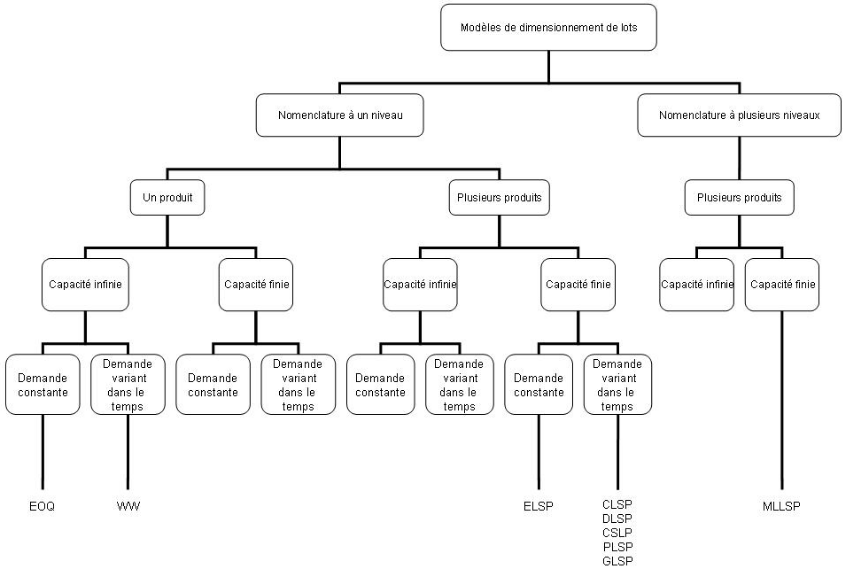
\includegraphics[scale=.5]{images/classification_dimensionnement.png}
			\caption{Exemple de classification des modèles de dimensionnement de lots \cite{cathy}}
			\label{fig:classification_dimensionnement_lots}
		\end{figure}
	\end{center}

	\newpage
	
	\section{Le \emph{Pigment sequencing problem} (PSP)}
	
	\subsection{Revue de littérature}
	Le PSP appartient à la catégorie des DLSP. En effet, il s'agit d'un problème où toute la capacité disponible sur cette période sera utilisée si un article est fabriqué. Nous présentons dans cette sous-section une brève revue de littérature des différents travaux effectués autour du PSP. \\
	\hspace*{.5cm} Miller et Wolsey \cite{miller_wolsey} ont formulé le DLSP avec des coûts de préparation indépendants de séquence comme un problème de réseau à flot. Ils ont présenté des formulations MIP pour les différentes extensions (avec \emph{backlogging}, avec stock de sûreté, avec stock initial). Plusieurs variantes et formulations MIP du DLSP ont été proposées et discutées par Pochet et Wolsey \cite{pochet_wolsey}. \\
	\hspace*{.5cm} Gicquel et al. \cite{gicquel_minoux_dallery} présentent une formulation et dérivent des inégalités valides pour le DLSP avec plusieurs articles et des coûts et temps de préparation séquentiels; laquelle est une extension du problème proposé par Wolsey \cite{wolsey}. Dans Gicquel et al. \cite {gicquel_miegeville_minoux_dallery}, les auteurs ont proposé une nouvelle manière de modéliser le DLSP avec plusieurs articles et des coûts et temps de préparation séquentiels; qui exploite le fait que les attributs physiques pertinents des articles, tels que la couleur, la dimension, le niveau de qualité. Cela leur a permis de réduire significativement le nombre des variables et des contraintes dans les modèles MIP.\\
	\hspace*{.5cm}Houndji et al. \cite{hvr_stockingCost} ont introduit une nouvelle contrainte globale, qu'ils ont appelée \emph{StockingCost} afin d'efficacement résoudre le PSP en programmation par contrainte. Les auteurs l'ont alors testée sur de nouvelles instances et les ont publiées sur CSPlib (Gent et Walsh \cite{gent_walsh}). Les résultats expérimentaux ont montré que le \emph{StockingCost} est plus efficace en filtrage tout en prenant en compte les autres techniques de décompositions généralement utilisées dans la communauté de la programmation par contrainte. \\
	\hspace*{.5cm} Plus récemment, Ceschia et al. \cite{ceschia} ont appliqué le recuit simulé sur le PSP. Ils ont implémenté une approche qui prend en charge à la fois la faisabilité de la solution et l'optimisation du coût. Dans le but d'illustrer leur méthode, ils ont introduit une procédure de recuit simulé afin de guider la recherche locale, qu'ils ont ensuite appliquée sur de nouvelles instances disponibles sur le bibliothèque Opthub \cite{opthub}.
	 
	\subsection{Description du problème}

		\label{sec:problem_description}
		Des différentes études \cite{ratheil_master} \cite{ceschia} déjà effectuées sur le PSP, nous pouvons le décrire comme une problème qui consiste à trouver un plan de production de plusieurs articles à partir d’une machine avec des coûts de transition. Les coûts de transition sont les coûts encourus lors du passage de la production de l’article $i$ à celui de l’article $j$ avec $i \neq j$. Le plan de production doit satisfaire les demandes des clients tout en :
	\begin{itemize}
		\item[•] respectant la capacité de production de la machine;
		\item[•] minimisant les coûts de stockage et de transition.
	\end{itemize}
	\hspace*{.5cm} On suppose que la période de production est suffisamment courte pour ne produire qu’au plus un article par période et que les demandes sont normalisées : la capacité de production de la machine est limitée à un article par
période et d($i$, $t$) $ \in $ {0, 1} avec $i$ l’article et $t$ la période.\\
	\hspace*{.5cm} Il s’agit d’un problème de planification de production ayant les caractéristiques suivantes : un horizon de planification discret et fini ; des contraintes de capacité ; une demande statique et déterministe ; multi-item et small bucket, des coûts de transition; un seul niveau; sans shortage.\\

	\textbf{\textsl{Illustration}} : Soit un problème avec les données ci-dessous : \\
	\begin{itemize}
		\item[•] Nombre d’articles : $NI = 2$;
		\item[•] Nombre de périodes : $NT = 5$;
		\item[•] Demande par période. Soit d($i$, $t$) la demande de l’article $i$ à la période $t$ : $d(1, t) = (0, 1, 0, 0, 1)$ et $d(2, t) = (1, 0, 0, 0, 1)$;
		\item[•] Coût de stockage. Soit $h(i)$ le coût de stockage de l’article $i$ : $h(1) = h(2) = 2$;
	\end{itemize}
	Soit \emph{xT} le plan de production qui représente une solution potentielle du problème. Il s’agit d’un tableau de dimension \emph{NT} , contenant à son indice $t$ (avec $t  \in  {1...NT}$) l’article $i$ à produire. Une solution admissible du problème est : $ xT = (2, 1, 2, 0, 1)$ avec un coût de $ q(2, 1) + q(1, 2) + q(2, 1) + 2 * h(2) = 15 $. La solution optimale est : $ xT = (2, 1, 0, 1, 2)$ avec un coût de $q(2, 1) + q(1, 2) + h(1) = 10$.
		
		\subsection{Modèles et formulations}
		Différents modèles ont été proposés afin de représenter, modéliser et résoudre le PSP. Il s'agit des modèles de programmation mixte en nombres entiers ou MIP (au nombre de 3) proposés par Pochet et Wolsey \cite{pochet_wolsey}, considérés comme l'état de l'art des méthodes de résolution exactes sur les problèmes de dimensionnement de lots en particulier celui du PSP, du modèle CP et du modèle SA. Nous présentons donc ici le premier modèle MIP dont les deux derniers sont une reformulation, le modèle CP ainsi que le modèle SA.
		\subsubsection{Modèle MIP 1}
		
		Le modèle MIP 1 \cite{pochet_wolsey} tel qu'exposé par Pochet et Wolsey se présente comme suit:
		\begin{eqnarray}
			min \sum_{i,j,t} q^{i,j}ch_{t}^{i,j} + \sum_{i,t} h^{i} s_{t}^{i} \\
			s_{0}^{i} = 0, \forall i \\
			x_{t}^{i} + s_{t-1}^{i} = d_{t}^{i} + s_{t}^{i}, \forall i,t \\
			x_{t}^{i} \leq y_{t}^{i}, \forall i,t \\
			\sum_{i} y_{t}^{i} = 1 , \forall t \\
			\chi_{t}^{i,j} = y_{t-1}^{i} + y_{t}^{j} - 1, \forall i,j,t \\
			x,y,\chi \in \{0,1\}, s \in N, i \in \{0..NI\}, t \in \{1..NT\}
		\end{eqnarray}
		
		avec les variables de décisions suivantes: \\
		\begin{itemize}
			\item[-] $x_{t}^{i}$ : variable binaire de production qui vaut 1 si l’article $i$ est produit à la période $t$ et 0 sinon ;
			\item[-] $y_{t}^{i}$ : variable binaire de setup qui vaut 1 si la machine est préparée pour la production de l’article $i$ et 0 sinon ;
			\item[-] $s_{t}^{i}$ : variable entière de stockage qui contient le nombre d’articles $i$ stockés à la période $t$ ; 
			\item[-] $\chi_{t}^{i,j}$ : variable binaire de transition qui vaut 1 si à la période $t$, on est passé de la production de l’article $i$ à l’article $j$ et 0 sinon.
		\end{itemize}
		\vspace*{.3cm}
	\hspace*{.5cm} L'objectif est de minimiser la somme des coûts de stockage et des coûts de transition et est exprimé par la contrainte (1). La contrainte (2) rappelle qu'il n'y a pas de stock initial. La contrainte (3) exprime la règle de la conservation de flot. La contrainte (4) vise à forcer la variable de setup $y_{t}^{i}$ à prendre la valeur 1 s’il y a production de l’article $i$ à la période $t$. La contrainte (5) s'assure qu'il y a toujours un article qui est préparé. En accord avec la fonction objectif, $y_{t}^{i}$ va prendre la valeur qui minimise le coût de transition. En général s’il n’y a pas de production à la période $t$,
$y_{t}^{i} = y_{t-1}^{i}$ ou $y_{t}^{i} = y_{t+1}^{i}$
mais parfois il peut être intéressant de préparer la machine pour un article intermédiaire sans le produire. La contrainte (6) assigne les valeurs aux variables de transition.
En effet, si $y_{t-1}^{i}$ et $y_{t}^{i}$ valent 1 alors $\chi_{t}^{i,j}$ est obligé de prendre la valeur 1 et sinon $ch_{t}^{i,j}$ serait égale à 0 grâce à la fonction objectif qui minimise le coût de transition.
		
		\subsubsection{Modèle CP}
		Dans ce modèle \cite{ratheil_master}, l’objectif est d’attribuer à chacune des demandes, une période qui respecte la date limite de satisfaction de la demande. On note $date(p) \in [1,...,T],\ \forall p \in [1,...,n]$ la période dans laquelle la demande $p$ a été satisfaite, $dueDate(p) \in [1,...,T]$ la date limite de la demande $p$ et $I(p)$ l'article correspondant à la demande $p$. Afin de s'assurer de la faisabilité de la solution, les principales contraintes sont les suivantes:
		\begin{eqnarray}
			date(p) \leq duedate(p), \forall p \\
			alldifferent(date)
		\end{eqnarray}
		
		dans lesquelles:
		\begin{itemize}
			\item[-] Equation 8: chaque demande doit être satisfaite avant sa date limite;
			\item[-] Equation 9: Puisque la capacité d'une machine est limitée à 1, chaque demande doit être satisfaite à différente période.
		\end{itemize}
		Il est possible de modeler la partie des coûts de transition comme un ATSP, chaque demande représente une ville qui doit être visitée et les coûts de transition sont les distances entre deux villes. Ainsi, on ajoute une demande artificielle $n+1$ de sorte que $date(n+1) = T+1$ avec $q^{I(p), I(n+1)} = q^{I(n+1), I(p)} = 0, \forall p \in [1,...,n]$. On note alors $successor(p), \forall p \in [1,...,n]$, la demande satisfaite juste après la satisfaction de la demande $p$. Les contraintes suivantes additionnelles peuvent être alors ajoutées:
		\begin{eqnarray}
			circuit(successor) \\
			date(p) \leq date(successor(p)), \forall p \in [1,...,n]
		\end{eqnarray}
		dans lesquelles:
		\begin{itemize}
			\item[-] Equation 10: il garantit l'existence d'un circuit hamiltonien;
			\item[-] Equation 11: la demande $p$ doit être satisfaite avant ses successeurs.
		\end{itemize}
		
		Enfin, l'objectif est de minimiser les coûts de stockage et les coûts de transition.
		\[
			\sum_{p}{(dueDate(p)-date(p))} * h_{I(p)} + \sum_{p}{q^{I(p),I(successor(p))}}
		\]
		
	
		\subsubsection{Modèle SA}
		Dans ce modèle \cite{ceschia}, la procédure de recuit simulé conduit à chaque itération à une action aléatoire en utilisant une distribution uniforme. Comme toujours en recuit simulé, l'action est toujours acceptée si elle est facteur d'amélioration. Dans le cas contraire, elle est acceptée, si elle est basée sur une distribution en temps croissant de façon exponentielle. Dans le détail, une mauvaise action est acceptée avec une probabilité de $e^{-\Delta/T}$ où $\Delta$ est la différence du coût total induit par l'action et $T$ est la température. La température commence à une valeur $T_{0}$ et est multipliée par $\alpha$ (avec $0 < \alpha < 1$), après un nombre fixé d'échantillons $n_{s}$, selon la procédure de refroidissement géométrique standard du recuit simulé. \\
		\hspace*{.5cm} Dans le but d'accélérer les premières étapes de la procédure de recuit simulé,  Ceschia et al. ont utilisé un mécanisme de \emph{cut-off} (Johnson et al. \cite{johnson}). Ils ont ajouté un nouveau paramètre $n_{a}$ représentant le nombre maximal d'actions acceptées à chaque niveau de température. Ainsi, la température diminue lorsque la première des deux conditions suivantes est remplie : ($i$) le nombre d'actions échantillonnées atteint $n_{s}$, ($ii$) le nombre d'actions acceptées atteint $n_{a}$. \\
		\hspace*{.5cm} Le critère de terminaison est basé sur le nombre total d'itérations $I_{max}$, plutôt que sur un seuil de température. De cette manière, le temps d'exécution est approximativement le même pour toutes les configurations des paramètres.
		
	\section{Les algorithmes génétiques}
		
	Les algorithmes génétiques (GAs) sont des algorithmes d’exploration fondés sur les mécanismes de la sélection naturelle et de la génétique \cite{holland1} \cite{holland2}. Ils utilisent à la fois les principes de la survie des structures les mieux adaptées, et les échanges d’informations aléatoires, parfois guidés, pour former un algorithme d’exploration qui possède certaines des caractéristiques de l’exploration humaine. Ils ont été proposés pour la première fois et sont devenus populaires à travers les travaux de John Holland au début des années 1970, et particulièrement son livre \emph{Adapation in Natural an Artificial Systems} (1975). Holland présenta les GAs comme une abstraction de l'évolution biologique et des concepts théoriques à l'adaptation pour les GAs dans son livre. Il introduisit un formalisme afin de prédire la qualité de la prochaine génération, plus connue comme le théorème des schémas de Holland.
	
	\subsection{Concepts de base}
	Les AGs constituent une classe de stratégies de recherche réalisant un compromis entre l’exploration et l’exploitation. Ils représentent des méthodes qui utilisent
un choix aléatoire comme outil pour guider une exploration intelligente dans l’espace des paramètres codés. Ce sont des algorithmes itératifs de recherche globale dont l’objectif est d’optimiser une fonction prédéfinie appelée fonction coût ou fonction « fitness ».
	Les algorithmes génétiques emploient un vocabulaire emprunté à la génétique naturelle. Ils travaillent sur un ensemble d’individus appelé population. Un individu a deux représentations appelées phénotype et génotype. Le phénotype représente une solution potentielle du problème à optimiser en utilisant la formulation originale du problème. Le génotype donne une représentation codée
d’une solution potentielle sous la forme d’un chromosome. Un chromosome est formé de gènes disposés en une succession linéaire et chaque gène peut prendre plusieurs
valeurs appelées allèles. Par exemple, un chromosome se compose d’une succession de 0 et de 1 (c.-à-d. une chaîne binaire), et la valeur pour une certaine position correspond à "on" (la valeur = 1) ou à "off" (la valeur = 0) d’un certain dispositif. Des formes plus compliquées, telles qu’un ordre des symboles et une permutation des alphabets, sont choisies pour décrire les chromosomes du problème à optimiser. Chaque individu a une fonction objectif f (fonction « fitness ») qui mesure l’adaptation de l’individu à son environnement local. La théorie darwinienne indique que, parmi des individus d’une population, celui qui est le mieux adapté à l’environnement local a le plus de chance de survivre et d’avoir un plus grand nombre de descendants : c’est la règle de la « survie du plus fort ». Ainsi, la
fonction objectif f du problème d’optimisation joue le rôle d’un critère d’adaptation. Un des points les plus importants des algorithmes génétiques est la flexibilité dans la fonction objectif.

	\subsection{Fonctionnement}
	
	L'algorithme \ref{algo:algo_genetique_standard} présente le principe de fonctionnement de l'algorithme génétique simple.\\
	 
	\begin{algorithm}[H]
 	\caption{Algorithme génétique standard \cite{Goncalves}}
 	\label{algo:algo_genetique_standard}
 	%\KwData{this text}
 	%\KwResult{how to write algorithm with \LaTeX2e }
 	%initialization\;
 	Générer la population initiale $P_{i}$ \\
 	Évaluer la population $P_{i}$ \\
 	\While{le critère de terminaison n'est pas satisfait}{
 	 Sélectionner les éléments de $P_{i}$ à copier dans $P_{i+1}$ \\
 	 Appliquer le croisement aux éléments de $P_{i}$ et les mettre dans $P_{i+1}$ \\
 	 Appliquer la mutation aux éléments de $P_{i}$ et les mettre dans $P_{i+1}$ \\
 	 Évaluer la nouvelle population $P_{i+1}$ \\
 	 $P_{i}$ = $P_{i+1}$
 	}
	\end{algorithm}
	
	\vspace*{1cm}
	Cet algorithme \ref{algo:algo_genetique_standard} est explicité plus en détails à l'aide de la figure \ref{fig:genetic_algo_flowchart}.
	
	\begin{figure}[!h]
		\begin{center}
			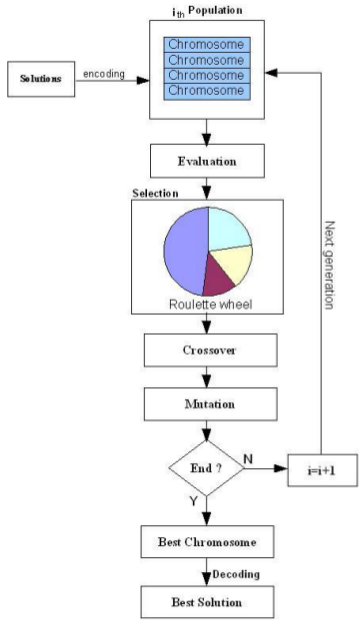
\includegraphics[scale=.5]{images/genetic_algo_flowchart.png}
			\caption{Diagramme d'un algorithme génétique standard \cite{denny}}
			\label{fig:genetic_algo_flowchart}
		\end{center}
	\end{figure}
	
	\newpage
	
	\subsection{Les opérateurs}
		Un algorithme génétique simple utilise les trois opérateurs suivants : la sélection, le croisement et la mutation.
		\subsubsection{L’opérateur de sélection}
		La sélection est un processus dans lequel des individus d’une population sont choisis selon les valeurs de leur fonction coût ou «  fitness  » pour former une nouvelle population. Les individus évoluent par des itérations successives de la sélection, appelées générations. Chaque individu est sélectionné proportionnellement à sa fonction « fitness », donc, un individu avec une fonction « fitness »
plus élevée aura plus de chance d’être sélectionné qu’un autre avec une valeur de « fitness » inférieure. Cette fonction peut être envisagée comme une mesure de profit ou de qualité qu’on souhaite maximiser. Un opérateur simple de sélection est la technique de la roulette pondérée où chaque individu d’une population
occupe une surface de la roulette proportionnelle à la valeur de sa fonction « fitness ». Pour la reproduction, les candidats sont sélectionnés avec une probabilité proportionnelle à leur «  fitness  ». Pour chaque sélection d’un
individu, une simple rotation de la roue donne le candidat sélectionné. Cependant cette sélection n’est pas parfaite. En effet, le risque de favoriser un individu ou un petit ensemble d’individus constitue un inconvénient qui risque d’appauvrir la diversité de la population.
	\subsubsection{L’opérateur de croisement}
	Le croisement est un opérateur de recombinaison. Les individus d’une population sont couplés au hasard par paires représentant les parents. Chaque paire d’individus
subit le croisement décrit comme suit : le croisement opère sur les génotypes (c.-à-d. les chromosomes) de deux individus appelés parents. Il produit de nouveaux individus (généralement deux) appelés enfants dont les gènes sont hérités de l’un ou/et de l’autre parent. Ceci peut être fait en dédoublant chacun des deux chromosomes dans des fragments et en les recombinant pour former de nouveaux chromosomes.
	\begin{description}
		\item[\textsl{Le croisement à un point :}] Si le génotype est une chaîne binaire de longueur n. Le croisement à un point place un point de croisement au
hasard. Un enfant prend une section avant le point de croisement d’un parent et prend l’autre section après le point de croisement de l’autre parent puis recombine les deux sections pour former une nouvelle chaîne binaire. L’autre enfant se construit inversement. 
		
		\item[\textsl{Le croisement à deux points :}]Le croisement à deux points place deux points de croisement au hasard, et prend une section entre les points d’un parent et les autres sections en dehors des points de l’autre parent puis les recombine. 
	
		\item[\textsl{Le croisement uniforme :}]Ce type de croisement a été proposé par Syswerda \cite{Syswerda}. Il consiste à choisir avec la même probabilité un allèle de l’un ou de l’autre parent, pour transmettre sa valeur à la même position, aux enfants. 
	
	\end{description}
	
	\subsubsection{L'opérateur de mutation}
	
	La mutation opère sur le génotype d’un seul individu. Elle correspond, dans la nature, à une « erreur » qui se produit quand le chromosome est copié et reproduit. Dans une approche numérique, pour une chaîne binaire, elle consiste par exemple à faire pour un allèle un échange entre le « 0 » et le « 1 ». Si des copies exactes sont toujours garanties, alors le taux de mutation est égal à zéro. Cependant, dans la vie réelle, l’erreur de copie peut se produire dans diverses circonstances comme sous l’influence d’un bruit. La mutation change les valeurs de certains gènes avec une faible probabilité. Elle n’améliore pas, en général, les solutions, mais elle évite une perte irréparable de la diversité.
	
	\subsection{Application des algorithmes génétiques aux problèmes d'optimisation}
	
	Les algorithmes génétiques ont été largement utilisés ces dernières années \cite{jawahar}. L’utilisation des AGs dans de nombreux domaines a fait ses preuves, notamment dans des problèmes combinatoires tels que les problèmes d’ordonnancement \cite{davis} et les problèmes de collecte et de distribution. Les problèmes d’ordonnancement d’un atelier classique de type Job-Shop (JSP) ont notamment été largement étudiés et résolus par les AGs \cite{boukef}. D’autres algorithmes hybrides ont été aussi proposés \cite{cavalieri}. La difficulté principale dans la résolution de ces types de problèmes résulte dans la façon avec laquelle ils sont représentés sous forme algorithmique. Dans cette phase, la définition du chromosome représente le point le plus important dans la recherche génétique. Plusieurs approches de représentation et différents types d’opérateurs d’AGs ont été proposés, pour résoudre ces problèmes.
	
	\section*{Conclusion}
	\addcontentsline{toc}{section}{Conclusion}
	Le dimensionnement de lots en planification de production est un important défi pour les entreprises industrielles. Il consiste à trouver un plan de production qui satisfait aux contraintes spécifiques relatives au système de production. Le PSP constitue en effet une variante NP-Difficile de ces types de problèmes. Plusieurs méthodes peuvent servir à résoudre ce problème. Au nombre de ces méthodes, figurent les algorithmes génétiques. Les AGs, à travers l'exploration et l'exploitation de l'espace de recherche ont permis de résoudre bon nombre de problèmes d'optimisation par le passé. Nous avons également présenté le PSP ainsi que les modèles et leur formulation qui ont été utilisés dans sa résolution.	Dans le partie suivante, nous décrivons les outils de test, les méthodes de résolution proposées ainsi que les algorithmes associés.


\chapter{Matériel et solutions}{\label{chap:materiel_et_solutions}}
	\section*{Introduction}
	\addcontentsline{toc}{section}{Introduction}
	L'étude des problèmes de dimensionnement de lots au cours de décennies de recherche a permis de tester différentes méthodes de recherche à ces types de problèmes. L'étude du "Pigment Sequencing Problem" (PSP) n'échappe pas à la règle. Dans ce chapitre, nous présentons dans un premier temps, le modèle utilisée dans notre étude afin de représenter les instances de PSP, ensuite les aspects généraux ou communs à nos deux approches heuristiques basées sur les algorithmes génétiques; puis dans un second temps, nous décrivons ces deux méthodes de recherche en nous appuyant sur les algorithmes implémentés.
	
	\section{Environnement de test} 
		
		\subsection{Matériel}
		Pour l'implémentation de nos tests, nous avons travaillé sur un ordinateur présentant les caractéristiques suivantes :\\
		\begin{itemize}
			\item[•] Système d'exploitation: Linux Ubuntu 16.04 LTS; \\
			\item[•] Processeur: Intel®  Core \up{\textsc{TM}} i7 CPU L 640 @ 2.13GHz x 4; \\
			\item[•] Mémoire: 3,7 Gio;\\
			\item[•] Type du système d'exploitation: 64 bits.\\
		\end{itemize}
		\subsection{Langage de programmation}
		Le langage de programmation utilisée afin d'implémenter notre solution est le langage \emph{Python} dans sa version Python 3.5. \emph{Python} est un puissant langage de programmation interprété qui apparaît de plus en plus comme une alternative crédible et intéressante dans le domaine de l'intelligence artificielle, tant il présente des qualités quant à sa robustesse, sa rapidité, sa portabilité, sa facilité de prise en main, sa rigueur et sa caractéristique de langage Open source.  
		
		\subsection{Données de test}
		
		Afin de tester nos deux solutions, nous commençons dans un premier temps par utiliser un ensemble de 10 instances proposées par Houndji et al. auxquelles ils ont appliqué le CP. Ces instances sont caractérisées par un nombre de périodes \emph{NT} = 20 et un nombre d'articles \emph{NI} = 5. Les résultats seront comparés à ceux obtenus par Houndji et al. dans leur application de l'approche CP à ces instances. \\
		\hspace*{.5cm} Dans un second temps, nous appliquons nos deux solutions à 6 autres instances proposées par Ceschia et al \cite{ceschia} dans leur bibliothèque Opthub. En effet, dans le but de tester leur approche de solution basée sur le recuit simulé aux instances de PSP, Ceschia et al ont  développé un générateur paramétré produisant de nouvelles instances plus complexes. Le générateur travaille de sorte que l'instance produite est faisable, c'est à dire qu'elle satisfait aux contraintes de \emph{NoBacklog}. Nous testons donc notre approche de solution à ces nouvelles instances complexes et comparons nos résultats à ceux obtenus par Ceschia et al dans leur application du recuit simulé à ces instances. \\
		\hspace*{.5cm} Dans les deux cas, nos critères d'analyse sont de deux ordres. Premièrement, nous les avons analysées sous l'angle de la performance en temps. Il s'agit de voir comment ces algorithmes arrivent à répondre aussi rapidement que possible nos instances de PSP.  Le second angle d'analyse s'est porté sur la performance en terme de la qualité de la solution trouvée. Nous avons calculé l'écart entre la solution trouvée et la solution optimale connue dans la littérature.
		
		\subsection{Paramètres de test}
		Les paramètres de test utilisés afin d'effectuer les tests sont présentés comme suit selon que le programme soit HCM-PGA ou HFC-PGA:

		\begin{enumerate}
			\item HCM-PGA \\
				\begin{itemize}
					\item[-] Taille de la population : 25 individus par processus ;
			        \item[-] Probabilité de mutation : 5\%;
			        \item[-] Probabilité de croisement : 80\%;
			        \item[-] Nombre de migrants : 1 individu;
		 	        \item[-] Nombre de processus esclaves : 2 processus;
			        \item[-] Nombre de processus principaux : 2 processus;
			        \item[-] Nombre de générations avant migration : 0 génération (la migration intervient après une convergence).
				\end{itemize}
				\vspace*{.5cm}
			\item HFC-PGA \\
				\begin{itemize}
					\item[-] Taille de la population : 25 individus par processus ;
			        \item[-] Probabilité de mutation : 5\%;
			        \item[-] Probabilité de croisement : 80\%;
			        \item[-] Nombre de migrants : 1 individu;
			        \item[-] Nombre de processus principaux : 2 processus;
			        \item[-] Nombre de générations avant migration : 0 génération (la migration intervient après une convergence).
				\end{itemize}
		\end{enumerate}
		Ces paramètres de test sont les valeurs qui nous sont parues maximisant la qualité des solutions trouvées par chacun des algorithmes.	
	
	\section{Modèle et formulation utilisés}
	Dans le but de modeliser et de formuler les instances de PSP, nous nous sommes servi de la première formulation en programmation en nombres entiers (MIP1). Nous rappelons ici ce modèle. 
	
	\begin{eqnarray}
		min \sum_{i,j,t} q^{i,j}ch_{t}^{i,j} + \sum_{i,t} h^{i} s_{t}^{i} \\
		s_{0}^{i} = 0, \forall i \\
		x_{t}^{i} + s_{t-1}^{i} = d_{t}^{i} + s_{t}^{i}, \forall i,t \\
		x_{t}^{i} \leq y_{t}^{i}, \forall i,t \\
		\sum_{i} y_{t}^{i} = 1 , \forall t \\
		\chi_{t}^{i,j} = y_{t-1}^{i} + y_{t}^{j} - 1, \forall i,j,t \\
		x,y,\chi \in \{0,1\}, s \in N, i \in \{0..NI\}, t \in \{1..NT\}
	\end{eqnarray}
		
		avec les variables de décisions suivantes: \\
		\begin{itemize}
			\item[-] $x_{t}^{i}$ : variable binaire de production qui vaut 1 si l’article i est produit à la période t et 0 sinon ;
			\item[-] $y_{t}^{i}$ : variable binaire de setup qui vaut 1 si la machine est préparée pour la production de l’article i et 0 sinon ;
			\item[-] $s_{t}^{i}$ : variable entière de stockage qui contient le nombre d’articles i stockés à la période t ; 
			\item[-] $\chi_{t}^{i,j}$ : variable binaire de changeover qui vaut 1 si à la période t, on est passé de la production de l’article i à l’article j et 0 sinon.
		\end{itemize}
	
	\section{Aspects généraux aux deux méthodes de recherche proposées}
	\subsection{Représentation génétique}
	Différentes représentations peuvent être utilisées avec les techniques évolutionnaires telles que les algorithmes génétiques. La représentation la plus simple pour les algorithmes génétiques est celle utilisée par John Holland: une chaîne de bits. Une chaîne de bits est connue comme un chromosome, et chaque bit est un gène. En début d'étude, nous avons donc commencé par représenter un chromosome en chaîne de bits. \\
	\textsl{\textbf{Exemple}}:\\
	\hspace*{.5cm} En suivant l'exemple d'une instance de PSP en page \pageref{sec:problem_description}, nous pouvons représenter un chromosome conformément à la figure \ref{fig:init_gene_repr}.
	
	\begin{figure}[h]
		\begin{center}
			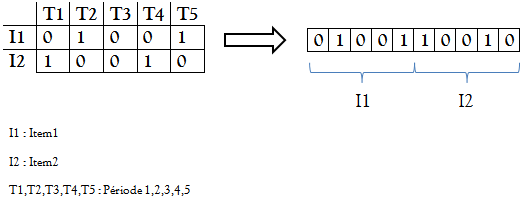
\includegraphics[scale=.5]{images/init_gene_repr.png}
			\caption{Représentation génétique initiale}
			\label{fig:init_gene_repr}
		\end{center}
	\end{figure}
	
	Autrement dit:
	\begin{center}
		$ch_{T} = \{(x_{1,1}),..., (x_{1,t+1}),..., ( x_{1,T}), (x_{i+1,1}),...,(x_{i+1, t+1}),..., (x_{i+1,T}),..., (x_{I,T})\}$ \\
	\end{center}
	\hspace*{.5cm} où $x_{it}$ est la variable booléenne qui indique la production ou non d'un article \emph{i} en période \emph{t}.  \\
	\\
	\hspace*{.5cm} Dans cette représentation, un chromosome est une chaîne de bits (0 et 1) qui indique la production ou non d'un article \emph{i} et de longueur \emph{nItems * nTimes} (où \emph{nItems} est le nombre d'articles et \emph{nTimes} est le nombre de périodes). Ainsi, l'article 1 est produit dans les périodes 2 et 5; et l'article 2 est produit dans les périodes 1 et 4. Le chromosome représenté ci-dessus est ainsi un plan de production qui satisfait aux contraintes du système de production spécifiques à cette instance du problème. Toutefois, au cours de notre étude, une seconde représentation nous est apparue plus cohérente et facilement manipulable. Cette représentation génétique est présentée à la figure \ref{fig:adopt_gene_repr} et étudiée par Mirshekarian et al. \cite{suer}.
	
	\begin{figure}[!h]
		\begin{center}
			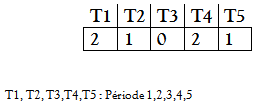
\includegraphics[scale=.5]{images/adopt_gene_repr.png}
			\caption{Représentation génétique adoptée}
			\label{fig:adopt_gene_repr}
		\end{center}
	\end{figure}
	
	Dans cette représentation, un chromosome est une suite d'entiers correspondant aux articles produits et de longueur \emph{nTimes}. La longueur réduite de ce chromosome réduit dans le même temps la complexité du parcours du chromosome lors des implé-mentations.
	\subsection{Initialisation}
	Le processus d'initialisation consiste à construire la population initiale; c'est à dire celle à partir de laquelle se feront les opérations de sélection, croisement ou encore mutation afin de la faire évoluer sur des générations. L'initialisation au niveau des algorithmes génétiques se fait de manière aléatoire dans l'optique de trouver des individus suffisamment différents capables de constituer une population diverse dans le but de largement couvrir l'espace de recherche. \\
	\hspace*{.5cm} Une autre approche consiste à créer les individus devant composer la population initiale en se servant de stratégies de recherche déterministes et informés munis de fonctions d'évaluation suffisamment précises menant à des bonnes solutions. Notre approche a été donc d'utiliser une stratégie de recherche en l’occurrence le "Hill Climbing" dotée d'une fonction d'évaluation afin de déterminer lequel des fils à considérer.\\
	\hspace*{.5cm} \textbf{\textsl{Principe:}}\\
	Le principe d'initialisation de la population est le suivant : remplir un chromosome en commençant par le dernier gène et en finissant par le premier. Cela permet de s'assurer de la faisabilité des solutions que nous trouvons au bout du processus. Ainsi, pour chaque gène visité, nous disposons de la liste des allèles qui peuvent prétendre occuper ce dernier, nous pouvons alors choisir l'allèle qui minimise le "fitness" du chromosome en train d'être constitué.\\
	\hspace*{.5cm} \textbf{\textsl{Algorithme:}}\\	
	L'algorithme \ref{alg:generation_pop_init} détaille le processus de génération de la population initiale: \\
	
	\begin{algorithm}[H]
		\caption{Processus de génération de la population initiale}
		\label{alg:generation_pop_init}
 		\KwData{instance de PSP à traiter, taille de la population}
 		\BlankLine
 		\KwResult{Population initiale constituée}
		\BlankLine 		
		$queue \gets []$
		\BlankLine
		$noeud \gets nouveauNoeud()$ \\
		\BlankLine
 		\While{taille(populationInitiale) est inférieure à taillePopulation}{
 			\BlankLine
 			\eIf{noeud.chromosome est prêt}{
 				\BlankLine
 			 	populationInitiale.ajouter(noeud.chromosome)
 			 	\BlankLine
 			 }
 			 {
 			 	\BlankLine
 			 	$noeudFils \gets noeud.getSuccessors()$ \\
 			 	\BlankLine
 			 	noeudFils.trier(decroissant) \\
 			 	\BlankLine
 			 	queue.ajouter(noeudFils)
 			 	\BlankLine
 			 	\If {queue est vide}
 			 	{
 			 		\BlankLine
 			 		\Return populationInitiale
 			 		\BlankLine
 			 	}
 			 	\BlankLine
 			 	$noeud \gets  queue.dernier()$
 			 }	
	}
	\Return populationInitiale
	\end{algorithm}	
	L'algorithme \ref{alg:generation_successeurs} décrit la génération des successeurs d'un noeud donné.
	\begin{algorithm}
		\caption{Processus de génération des successeurs d'un noeud}
		\label{alg:generation_successeurs}
 		\KwData{noeud}
 		\BlankLine
 		\KwResult{liste des successeurs constituée}
		\BlankLine 		
		$successeurs \gets []$
		\BlankLine
		\For{ item $\gets$ nbItems $\KwTo$ 1}
		{
			\BlankLine
			\If{item.dernierDeadline $>=$ noeud.currentPosition}
			{
				\BlankLine
				noeudFils = copie(noeud)
				\BlankLine
				noeudFils.currentPosition -= 1
				\BlankLine
				successeurs.ajouter(noeudFils)
				\BlankLine
			}
		}
	\Return successeurs
	\end{algorithm}	
	
	\subsection{Opérateurs génétiques}
		\subsubsection{Sélection}
		
		La sélection est le processus qui consiste à choisir dans la génération actuelle, les chromosomes ou individus qui seront reproduits afin de former la prochaine génération. Différentes méthodes de sélection existent. On distingue entre autres, la sélection par tournoi et la sélection par "\emph{roulette wheel}". \\
		\hspace*{.5cm} Dans notre étude, nous choisissons de nous intéresser à la plus connue et commune d'entre les méthodes de sélection: le \emph{"Roulette Wheel"}. Dans la sélection par "\emph{roulette wheel}", les individus se voient attribués une probabilité d'être sélectionnés. Cette probabilité est directement proportionnelle à leur fonction d'évaluation. Les individus sont donc choisis aléatoirement en se basant sur leur probabilité et se reproduisent en générant des individus "\emph{fils}". Ces "\emph{fils}" sont ainsi de nouvelles solutions au problème et forme une nouvelle population.		
		
		\subsubsection{Croisement}
		
		Une fois les individus sélectionnés, intervient le croisement. Le croisement en un point a été choisi afin de reproduire ces individus. Cette forme de croisement reste une des plus simples et répandues. La figure \ref{fig:used_cross_over} présente une illustration du croisement appliqué à l'instance de PSP introduite à la page \pageref{sec:problem_description}. \\
		\begin{figure}[!h]
			\begin{center}
				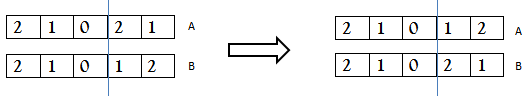
\includegraphics[scale=.5]{images/cross_over_fig.png}
				\caption{Illustration du croisement utilisé}
				\label{fig:used_cross_over}
			\end{center}
		\end{figure}
		
		\hspace*{.5cm} Le croisement se fait ainsi après la troisième période. Le croisement peut engendrer des individus qui, contrairement à la figure \ref{fig:used_cross_over}, ne respectent pas les contraintes de sytème en terme de \emph{shortage} ou de \emph{backlogging}. Il faut alors rendre ces individus à nouveau faisables avant de procéder à une quelconque mutation. L'algorithme \ref{alg:cross_over} présente le croisement implémenté dans le cadre de cette étude.\\
		
		\begin{algorithm}[H]
 		\caption{Algorithme de croisement utilisé}
 		\label{alg:cross_over}
 		\KwData{parent1, parent2, seuil\_probabilite}
 		\KwResult{child1 et child2}
 		\BlankLine
 		child1 $\gets$ $nouveau\ chromosome()$ \\
 		child2 $\gets$ $nouveau\ chromosome()$ \\
 		$probabilite \gets random(1,99)$ \\
 		\BlankLine
 		\If{probabilite $\leq$ seuil\_probabilite}
 		{
 			$nbGenes \gets NombreDeGenes(parent1)$\\
 			$indice\_gene \gets random(1, nbGenes)$\\
 			//$ Le \ nombre \ de \ genes \ du \ parent1 \ est \ le \ meme \ que \ celui \ du \ parent2 $\\
 			\For{ i $\gets$ 0 \KwTo nbGenes}
 			{
 				$gene1 \gets getGene(parent1, i)$ \\
 				$gene2 \gets getGene(parent2, i)$ \\
 				\eIf{i $\leq$ indice\_gene}
 				{
 					$child1.ajouterGene(gene)$ \\
 					$child2.ajouterGene(gene)$ \\
 				}
 				{
 					$child2.ajouterGene(gene)$ \\
 					$child1.ajouterGene(gene)$ \\
 				}
 			}
 		}
 		\Return{child1, child2}
		\end{algorithm}
		  
	\subsubsection{Mutation}
	Après la sélection et le croisement, une nouvelle population d'individus est prête. Certains ont été copiés directement et d'autres se sont reproduits par croisement. Dans le but de s'assurer que les individus ne sont pas exactement les mêmes, une mutation est appliquée à chacun des individus "\emph{fils}". A chaque gène, on attribue une chance de muter. Dans le cas, où la mutation se produit, la valeur du gène muté change de période. Un visuel de la mutation est présenté à la figure \ref{fig:used_mutation}. La mutation est un élément vital de la garantie d'une diversité au sein de la population. L'algorithme \ref{alg:mutation} détaille le processus utilisé afin de faire muter un chromosome. 
	
	\begin{figure}[!h]
		\begin{center}
			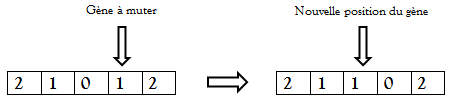
\includegraphics[scale=.5]{images/mutation_fig.png}
			\caption{Illustration de la méthode de mutation}
			\label{fig:used_mutation}
		\end{center}
	\end{figure}
	
	\begin{algorithm}[H]
 		\caption{Algorithme de mutation utilisée}
 		\label{alg:mutation}
 		\KwData{chromosome, seuil\_probabilite}
 		\KwResult{chromosome}
 		\BlankLine
 		$probabilite \gets random(1,99)$ \\
 		\BlankLine
 		\If{probabilite $\leq$ seuil\_probabilite}
 		{
 			\BlankLine
 			$nbGenes \gets NombreDeGenes(chromosome)$\\
 			\BlankLine
 			$indice\_gene \gets random(1, nbGenes)$\\
 			\BlankLine
 			$gene1 \gets getGene(chromosome, indice\_gene)$ \\
 			\BlankLine
 			//$ Le \ nombre \ de \ genes \ du \ parent1 \ est \ le \ meme \ que \ celui \ du \ parent2 $\\
 			\BlankLine
 			\For{ i $\gets$ indice\_gene \KwTo 0}
 			{
 				\BlankLine
 				$gene2 \gets getGene(chromosome, i)$\\
 				\BlankLine
 				\If{deadline(gene2) $>=$ indice\_gene}
 				{
 					\BlankLine
 					$deplacer(gene1, gene2, chromosome)$ \\
 					\BlankLine
 					$arret$
 					\BlankLine
 				}
 			}
 		}
 		\Return{chromosome}
		\end{algorithm}
	
	\subsection{Évaluation}
	L'évaluation dans notre étude, se réfère à la fonction objectif. Il s'agit de minimiser les coûts d'exploitation et de production. Deux types de coût sont à prendre en compte:
	\begin{itemize}
		\item[•] Les coûts de preparation ou \emph{setup} sont des coûts induits au moment d'un changement dans la configuration d'une ressource d'un type d'article à un autre. Il s'agit de perte potentielle de production durant la période de préparation, de force de travail additionnelle ou encore de ressources additionnelles brutes consommées durant la préparation.
		\item[•] Les coûts de stockage qui sont induits lors du conditionnement et d’entreposage.
	\end{itemize}
	L'algorithme \ref{alg:evaluation} explicite le processus suivi afin d'évaluer un chromosome.
	
	\begin{algorithm}[H]
 		\caption{Algorithme utilisé dans le processus d'évaluation d'un chromosome}
 		\label{alg:evaluation}
 		\KwData{chromosome, cout\_stockage, cout\_transition}
 		\KwResult{eval}
 		\BlankLine
 		$eval \gets 0$\\
 		$// On\ calcule\ le\ cout\ de\ stockage\ de\ chaque\ production$ \\
 		\For{gene in chromosome}{
 			\If{gene.value != 0}{		
 				$date\_limite \gets getDateLimite(gene)$ \\
 				$temp \gets (date\_limite\ -\ gene.periode) * cout\_stockage(gene.value)$ \\
 				$evaluation \gets evaluation\ +\ temp$ \\
 			}
 		}
 		$// On\ calcule\ le\ cout\ de\ transition\ de\ entre\ deux\ productions$ \\
 		\For{gene in chromosome}{
 			\If{gene.value != 0}{		
 				$next\_gene \gets getNextGene(chromosome)$ \\
 				\If{transition(gene, next\_gene) est vrai}{
 					$temp \gets cout\_transition(gene, next\_gene)$\\
 					$evaluation \gets evaluation\ +\ temp$
 				}
 			}
 		}
 		\Return{evaluation}
	\end{algorithm}
	
	\subsection{Terminaison}
	Deux moyens sont utilisés par lesquels les algorithmes génétiques se terminent. Habituellement, une limite est mise sur le nombre de générations après lesquelles le processus se termine. Avec certains problèmes, le processus de recherche se termine quand une solution particulière a été trouvée ou encore lorsque la plus haute valeur de "fitness" dans la population a atteint une valeur particulière. \\
	\hspace*{.5cm} Le critère de terminaison utilisé dans notre étude afin de terminer une recherche est le suivant : la recherche se termine lorsque l'algorithme converge sur un individu considéré comme une solution optimale. A cet optimal local, est appliqué une fonction de recherche locale afin de déterminer dans l'entourage immédiat de cet individu, un autre individu de meilleure qualité. Dans le cas, où un meilleur individu ne serait pas trouvé, la recherche s’arrête donc sur cet optimal local.
	
	\subsection{Fonction de faisabilité}
	Le croisement et la mutation sont tous des opérateurs génétiques qui produisent en sortie des chromosomes. En fonction du gène muté dans le cas de la mutation ou du point de croisement dans le cas du croisement, ces chromosomes peuvent ne pas être faisables; c'est-à-dire qu'ils ne représentent pas des solutions au problème à résoudre. Il importe donc de rendre à nouveau faisable. La fonction de faisabilité permet de rendre un chromosome ou individu à nouveau faisable. Afin d'y parvenir, nous avons réduit le surplus de production dans le cas d'un surplus et augmenter la quantité d'articles produits dans le cas d'un manque de production. L'algorithme \ref{alg:faisabilite} est celui utilisé dans cet objectif. 
	\\
	\begin{algorithm}[H]
 		\caption{Algorithme utilisé comme fonction de faisabilité}
 		\label{alg:faisabilite}
 		\KwData{chromosome, cout\_stockage, cout\_transition}
 		\KwResult{eval}
 		\BlankLine
 		$eval \gets 0$\\
 		$// On\ calcule\ le\ cout\ de\ stockage\ de\ chaque\ production$ \\
 		\For{gene in chromosome}{
 			\If{gene.value != 0}{		
 				$date\_limite \gets getDateLimite(gene)$ \\
 				$temp \gets (date\_limite\ -\ gene.periode) * cout\_stockage(gene.value)$ \\
 				$evaluation \gets evaluation\ +\ temp$ \\
 			}
 		}
 		$// On\ calcule\ le\ cout\ de\ transition\ de\ entre\ deux\ productions$ \\
 		\For{gene in chromosome}{
 			\If{gene.value != 0}{		
 				$next\_gene \gets getNextGene(chromosome)$ \\
 				\If{transition(gene, next\_gene) est vrai}{
 					$temp \gets cout\_transition(gene, next\_gene)$\\
 					$evaluation \gets evaluation\ +\ temp$
 				}
 			}
 		}
 		\Return{evaluation}
	\end{algorithm}
	
	\section{Algorithmes génétiques parallèles}	
	Les algorithmes génétiques sont des techniques de recherche qui ont été utilisées avec succès dans la résolution de problèmes dans différents disciplines. Cependant, la recherche permanente de performance dans l'exécution des algorithmes et le dévelop-pement constant d'ordinateurs toujours plus performants et parallèles ont conduit à l'émergence d'un type d'algorithmes génétiques plus performants que les algorithmes génétiques standards. A propos des algorithmes génétiques parallèles, on distingue généralement trois classes : les "\emph{master-slave} parallel genetic algorithms", les "\emph{ coarsed-grained} parallel genetic algorithms" et les "\emph{fine-grained} parallel genetic algorithms". Les "master-slave parallel genetic algorithms" sont le type le plus simple d'algorithmes génétiques parallèles. Elles consistent essentiellement à distribuer l'évaluation de la population globale entre plusieurs processeurs. Le processeur qui conserve la population et exécute l'algorithme génétique est le maître et les processus qui évaluent la population sont les esclaves. La figure \ref{fig:master_slave_ga} montre un schéma de l'algorithme génétique parallèle "master-slave". Nous nous intéressons dans notre étude aux deux autres types, plus compliqués mais également plus intéressants dans leur fonctionnement et performances.
	
	\begin{figure}[!h]
		\begin{center}
			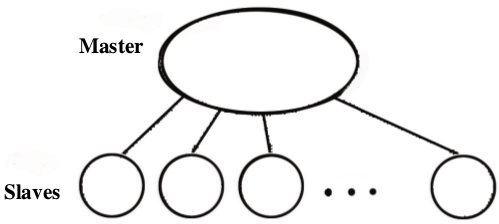
\includegraphics[scale=.3]{images/master_slave_ga.png}
			\caption{Schéma d'un algorithme génétique de type "master-slave" \cite{cant}}
			\label{fig:master_slave_ga}
		\end{center}
	\end{figure}
	
	\subsection{Algorithmes génétiques parallèles de type "\emph{coarse-grained}"}
	Les algorithmes génétiques de type "\emph{coarse-grained}" ou encore "\emph{modèle de l'île}" consiste en un ensemble de sous-populations qui échangent des individus de manière fréquente. Il s'agit probablement du type d'algorithmes génétiques le plus populaire bien qu'il nécessite de contrôler beaucoup de paramètres. La complète compréhension des effets de ces paramètres sur la qualité et la vitesse de recherche nous échappe encore. Cependant, Il a été démontré théoriquement que plus de sous-populations sont utilisées, leur taille peut être réduite sans sacrifier la qualité de la recherche. Vu que chaque processus s'exécute en parallèle, il en résulte une réduction du temps dédié aux calculs. Cependant, utiliser plus de sous-populations et donc de processus augmente la communication dans le système. Un compromis doit donc être effectué entre le temps de calculs et le temps de communication. L'implémentation des algorithmes génétiques parallèles soulève générale trois problématiques principalement sur la migration qui est l'échange d'individus entre processus. Il s'agit: de la fréquence de migration, du nombre d'individus à échanger, de la topologie des connections entre processus et de la méthode d'intégration des migrants.
	\subsubsection{Fréquence de migration}
	La migration affecte la qualité de la recherche et l'efficacité de l'algorithme en plusieurs points. Ainsi, de fréquentes migrations entraînent l'échange massif de potentiellement bons matériels génétiques, mais il affecte aussi négativement la performance dans le mesure où les communications sont coûteuses. La même chose se produit dans les topologies densément connectées où chaque processus communique avec les autres. Le but ultime des algorithmes génétiques parallèles est de trouver de bonnes solutions assez rapidement. Il est donc nécessaire de trouver l'équilibre entre le coût de la migration et l'augmentation des chances de trouver de bonnes solutions. \\
	\hspace*{.5cm} Afin d'implémenter l'algorithme, nous avons donné à l'utilisateur la possibilité d'entrer l'intervalle de générations en les migrations. Cependant, le comportement par défaut de l'algorithme est de migrer uniquement lorsque la population a convergé complètement.  
	\subsubsection{Nombre de migrants}
	La migration envoie un nombre prédéterminé d'individus d'un processus à ces processus voisins logiques sur le graphe de communications. Ces individus ou "\emph{migrants}" seront ainsi intégrés dans la population des processus auxquels ils ont été envoyés. Il est possible de choisir les "migrants" de façon aléatoire ou alors parmi les meilleurs individus de la population actuelle. La sélection aléatoire a l'avantage de disséminer plus de diversité et les chances d'explorer de nouvelles régions de l'espace de recherche peuvent être améliorées. La sélection des meilleurs individus peut aider à disséminer un matériel génétique qui a déjà été testé et qui serait donc intéressant. Dans la suite de notre étude, nous avons choisi d'échanger les meilleurs individus.
	\subsubsection{Topologie de connections}
	La topologie est également une importante partie des algorithmes génétiques de type \emph{"coarse-grained"}. En théorie, toute les topologies arbitraires peuvent être utilisées. Cependant, certains modèles sont fréquents. il s'agit : des topologies linéaires, des anneaux, des hypercubes. des densément connectés, des isolés. La topologie utilisée a été celle densément connectée présentée à la figure \ref{fig:topology_fig} 
	
	\begin{figure}[!h]
		\begin{center}
			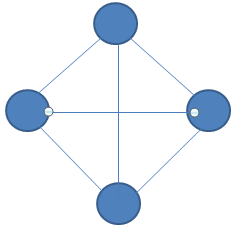
\includegraphics[scale=.3]{images/topology_fig.png}
			\caption{Topologie de connections utilisée}
			\label{fig:topology_fig}
		\end{center}
	\end{figure}
	
	\subsubsection{Méthode d'intégration des migrants}
 	Différentes alternatives existent pour incorporer les "\emph{migrants}". Deux d'entre elles sont récurrentes. Il s'agit: du remplacement aléatoire des individus de la population actuelle par les "\emph{migrants}" et du remplacement compétitif ou élitiste. Dans le remplacement aléatoire, les individus devant être remplacés sont désignés de manière aléatoire. Dans le remplacement compétitif, seules les individus avec les plus mauvais scores de "fitness" sont remplacés par les nouveaux arrivants. Un remplacement compétitif a été appliqué à notre programme. Il s'est agi d'identifier les plus mauvais chromosomes en terme de fitness et de les remplacer par les nouveaux arrivants.\\
 	\subsubsection{Algorithme hiérarchique entre \emph{coarse-grained} et \emph{master-slave}}
 	\hspace*{.5cm} Une fois, ces problématiques abordées, la question de l'implémentation rapide des algorithmes génétiques parallèles de type "\emph{coarse-grained}" revient. Une des réponses serait en effet de combiner ce type d'algorithmes génétiques parallèles avec un autre type, le "\emph{master-slave}" par exemple. On obtient alors un nouvelle classe d'algorithmes génétiques parallèles que sont les algorithmes génétiques parallèles hiérarchiques avec au niveau supérieur un algorithme génétique parallèle de type \emph{coarse-grained} et au niveau inférieur un algorithme génétique parallèle de type \emph{master-slave} comme le présente la figure \ref{fig:hierarchical_gene1_fig}. Il s'agit ainsi de cette combinaison que nous avons utilisée pour notre implémentation du programme et nos tests.
 	
	\begin{figure}[!h]
		\begin{center}
			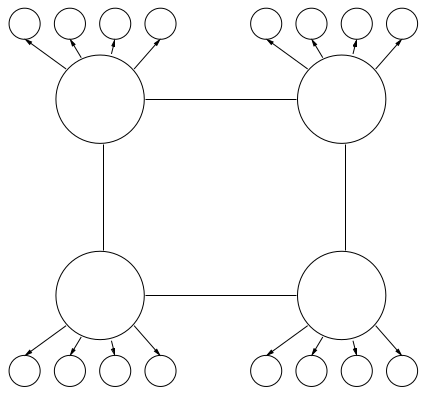
\includegraphics[scale=.3]{images/hierarchical_gene1_fig.png}
			\caption{Algorithmes génétiques parallèles et hierarchiques avec au niveau supérieur un algorithme génétique de type \emph{coarse-grained} et au niveau inférieur un algorithme génétique de type \emph{master-slave} \cite{cant2}}
			\label{fig:hierarchical_gene1_fig}
		\end{center}
	\end{figure} 	
 	
	\subsection{Algorithmes génétiques parallèles de type "\emph{fine-grained}"}
	les algorithmes génétiques parallèles de type "\emph{fine-grained}" ont seulement une population, mais la structure spatiale limite les interactions entre les individus. Un individu ne peut compétir et se reproduire qu'avec ses individus voisins. Vu que les voisinages se chevauchent, les bonnes solutions peuvent ainsi se disséminer à travers la population entière. Le choix le plus important dans l'implémentation de ce type d'algorithmes génétiques parallèles sont : la topologie de connections.
	\subsubsection{Topologie de connections}
	Différentes topologies de connections sont valables. Il s'agit entre autres des grilles 2-D, des hypercubes, le torus, le cube. Il est cependant répandu de placer les individus dans un algorithme génétique parallèle de type "\emph{fine-grained}" dans une grille 2-Dimension. En effet, dans la plupart des ordinateurs massivement parallèles, les éléments de traitement et de calculs sont connectés en suivant cette topologie. La figure \ref{fig:fine_grained_fig} présente la topologie utilisée afin d'implémenter l'algorithme génétique parallèle de type \emph{"fine-grained"}.
	
	\subsubsection{Principe de fonctionnement}
	Le principe de fonctionnement des algorithmes génétiques parallèles de type "\emph{fine-grained}" est différent de celui de type \emph{coarse-grained} et \emph{master-slave} est détaillé à l'algorithme \ref{alg:principe_fine_grained}. \\
	\\
	\begin{algorithm}[H]
 		\caption{Principe des algorithmes génétiques parallèles de type "\emph{fine-grained}" \cite{nayak}}
 		\label{alg:principe_fine_grained}
 		\BlankLine
 		\For{chaque nœud en parallèle}{
 		generer un individu de façon aléatoire
 		}
 		\BlankLine
 		\While{le critère de terminaison n'est pas satisfait}{
 			\For{chaque nœud en parallèle}{
 			evaluer le fitness de l'individu \\
 			obtenir la valeur de fitness des individus voisins \\
 			selectionner l'individu voisin dont la valeur de fitness est la plus grande \\
 			appliquer un croisement avec cet individu \\
 			muter l'individu qui en a résulté \\
 			}
 			Tester le critère de terminaison
 		}
	\end{algorithm}
	
	\begin{figure}[!h]
		\begin{center}
			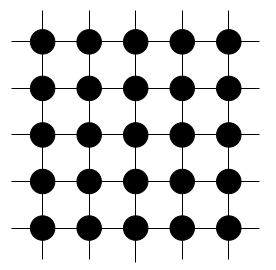
\includegraphics[scale=.3]{images/fine_grained_fig.png}
			\caption{Topologie utilisée en algorithme génétique parallèle de type "\emph{fine-grained}" \cite{cant2}}
			\label{fig:fine_grained_fig}
		\end{center}
	\end{figure} 
	
	\subsubsection{Algorithme hiérarchique entre \emph{fine-grained} et \emph{coarse-grained}}
	Des chercheurs ont combiné deux des méthodes de parallélisation produisant des algorithmes génétiques parallèles hiérarchiques. Certains de ces nouveaux algorithmes ajoutent un nouveau degré de complexité à des algorithmes déjà compliqués. On obtient alors des algorithmes génétiques parallèles hiérarchiques avec au niveau supérieur un algorithme génétique de type \emph{coarse-grained} et au niveau inférieur un algorithme génétique de type \emph{fine-grained} comme détaillé à la figure \ref{fig:hierar_fine_grained_fig}. Il s'agit en affet de notre deuxième proposition de méthode de résolution des instances de PSP que nous avons implémentée.
	
	\begin{figure}[!h]
		\begin{center}
			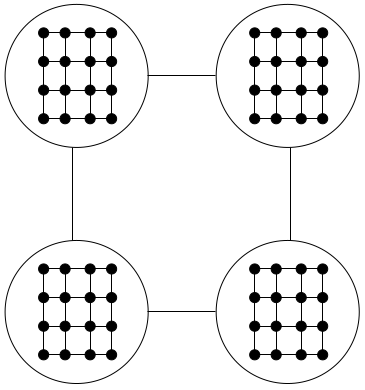
\includegraphics[scale=.3]{images/hierar_fine_grained_fig.png}
			\caption{Hiérarchie entre algorithmes génétiques parallèles de type \emph{fine-grained} et de type \emph{coarse-grained} \cite{cant2}}
			\label{fig:hierar_fine_grained_fig}
		\end{center}
	\end{figure} 
	\section{Autres implémentations}
	Au cours de notre étude de l'art et en implémentant nos deux méthodes de résolution proposées que sont les algorithmes génétiques parallèles et hiérarchiques \emph{coarse-grained} et \emph{master-slave} et les algorithmes génétiques parallèles et hiérarchiques \emph{coarse-grained} et \emph{fine-grained}, nous avons pu découvrir différentes fonctions annexes aux algorithmes génétiques qui permettent d'en améliorer la qualité. Il s'agit des méthodes d'hybridation \cite{Goncalves} et de table de hashage \cite{povinelli}.
	\subsection{Hybridation}
	L'hybridation consiste à combiner deux méthodes de recherche afin d'engendrer une nouvelle méthode de recherche dit \emph{hybride}. Les algorithmes génétiques facilitent l'hybridation avec les autres techniques de recherche locale afin d'obtenir la solution optimale. De façon basique, la recherche locale et les algorithmes génétiques sont complé-mentaires. Les algorithmes génétiques sont efficaces lorsqu'il s'agit de parcourir un espace de recherche global, dans la mesure où elles sont capables de rapidement trouver des régions prometteuses. Cependant, elles prennent relativement beaucoup de temps à trouver des optimums dans ces régions. La recherche locale est capable de trouver des optimums avec une grande précision. \\
	\hspace*{.5cm} Dans notre étude, il s'est agi de mettre au point un algorithme de recherche locale qui est utilisé à chaque fois que l'algorithme génétique converge sur une solution optimale afin de parcourir l'espace de recherche immédiat à cette solution et ainsi améliorer cette solution optimale.  \\
	\\
	\begin{algorithm}[H]
		%\label{alg:principe_fine_grained}
 		\caption{Algorithme de recherche locale d'une meilleure solution}
 		\KwData{individu à améliorer}
 		\BlankLine
 		\For{chaque gène du chromosome}{
 			\BlankLine
 			récupérer les coûts relatifs à la valeur de ce gène\\
 			\BlankLine
 			déterminer toutes les gènes à zéro respectant les contraintes liées à la valeur de ce gène.\\
 			\BlankLine
 			calculer le fitness du chromosome pour chaque gène à zéro\\
 			\BlankLine
 			choisir le gène à zéro qui maximise le fitness du chromosome \\
 			\BlankLine
 			insérer la valeur de l'item dans ce dernier gène\\ 
 			\BlankLine
 		}
	\end{algorithm}
	\vspace*{.5cm}
	Si on prend l'exemple du PSP en page \pageref{sec:problem_description} et qu'on applique cet algorithme au problème, on obtient la figure \ref{alg:principe_fine_grained}.
	
	\begin{figure}[!h]
		\begin{center}
			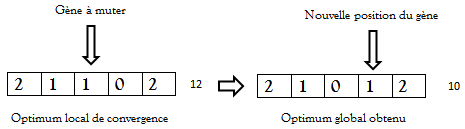
\includegraphics[scale=.6]{images/local_search_fig.png}
			\caption{Application de l'algorithme de recherche de meilleure solution à une chromosome}
			\label{fig:local_search_fig}
		\end{center}
	\end{figure} 
	
	\subsection{Table de Hash}
	Dans le processus de résolution des problèmes à l'aide algorithmes génétiques, au fur et à mesure que les générations passent, la population évolue et la diversité au sein de cette dernière diminue amenant les mêmes chromosomes à être régulièrement réévalués. Dans les faits, l'effort de calculs dépensé à évaluer le "\emph{fitness}" dépasse celui dépensé sur les opérateurs génétiques. En utilisant une table de hash afin de stocker les chromosomes récemment évalués, une amélioration significative des performances peut être constatée. Nous avons donc utilisé un dictionnaire ou tableau associatif afin de stocker ces derniers.
	
	\section*{Conclusion}
	\addcontentsline{toc}{section}{Conclusion}
	Cette deuxième partie a présenté le modèle utilisé dans la résolution du PSP ainsi que les aspects communs aux deux solutions proposées. Dans un second temps, nous avons présenté et détaillé deux approches heuristiques basées sur les algorithmes génétiques parallèles utilisées afin de résoudre le problème. La troisième partie sera l'occasion de tester nos deux approches et d'analyser les résultats afin de les comparer à l'état de l'art en la matière.

	
\chapter{Résultats et Discussion}
	\begin{abstract}
	Les deux approches basées sur les algorithmes génétiques présentées en chapitre \ref{chap:materiel_et_solutions} sont testées. Il en ressort que sur les instances proposées par Houndji \cite{houndji_thesis}, les deux approches parviennent à trouver des solutions très proches des solutions optimales assez rapidement. Elles ne parviennent cependant pas à en faire autant sur les grandes instances proposées par Ceschia \cite{ceschia}.
\end{abstract}

\section*{Introduction}
		\addcontentsline{toc}{section}{Introduction}
		Dans ce chapitre, nous testons les théories émises et analysons les résultats obtenus de tests afin de vérifier nos approches de solution du problème énoncées. A cette fin, nous présentons d'abord les données (instances) et paramètres de test. Ensuite, nous expérimentons nos solutions et à partir des résultats obtenus, nous comparons nos approches heuristiques basées sur les algorithmes génétiques à celles déjà appliquées à ce problème.
		
\section{Données et paramètres de test}
	\subsection*{Données de test}
Afin de tester nos deux solutions, nous commençons dans un premier temps par utiliser un ensemble de 20 instances des 100 proposées par Houndji et al. \cite{houndji_thesis} auxquelles ils ont appliqué la CP. Ces instances sont caractérisées par un nombre de périodes \emph{NT} = 20 , un nombre d'articles \emph{NI} = 5 et un nombre de demandes \emph{ND} = 20. Le choix de ces 20 instances s'est fait de la manière suivante: nous avons choisi les 5 premières instances des 100 proposées par Houndji, puis nous avons ensuite choisi 15 autres en veillant à combiner les instances sur lesquelles l'approche CP prenait le plus de temps et celles où elle en prenait le moins. Les résultats seront comparés à ceux obtenus par Houndji et al. dans leur application de l'approche CP à ces instances. \\
		\hspace*{.5cm} Dans un second temps, nous appliquons nos deux solutions à 6 autres instances des 27 proposées par Ceschia et al \cite{ceschia} dans leur bibliothèque Opthub. En effet, dans le but de tester leur approche de solution basée sur le recuit simulé aux instances de PSP, Ceschia et al (au même titre que Houndji dans son expérimentation du CP) ont  développé un générateur paramétré produisant de nouvelles instances plus grandes. Le générateur travaille de sorte que l'instance produite est faisable, c'est à dire qu'elle satisfait aux contraintes de \emph{NoBacklog}. Nous testons notre approche de solution sur ces nouvelles grandes instances et comparons nos résultats à ceux obtenus par Ceschia et al dans leur application du recuit simulé à ces instances. \\
		\hspace*{.5cm} Dans les deux cas, nos critères d'analyse sont de deux ordres. Premièrement, nous avons analysé les résultats sous l'angle de la performance en temps. Il s'agit de voir comment ces algorithmes arrivent à répondre aussi rapidement que possible nos instances de PSP.  Le second angle d'analyse s'est porté sur la performance en terme de la qualité de la solution trouvée. Nous avons calculé l'écart entre la solution trouvée et la solution optimale connue dans la littérature.
		
		\subsection*{Paramètres de test}
		Les paramètres de test utilisés afin d'effectuer les tests sont présentés comme suit selon que le programme implémente \emph{Hierarchical Coarse-grained and Master-slave Parallel Genetic Algorithm} (HCM-PGA) ou \emph{Hierarchical Fine-grained and Coarse-grained Parallel Genetic Algorithm}(HFC-PGA):

		\begin{enumerate}
			\item HCM-PGA \\
				\begin{itemize}
					\item[-] Taille de la population : 25 individus par processus ;
			        \item[-] Probabilité de mutation : 5\%;
			        \item[-] Probabilité de croisement : 80\%;
			        \item[-] Nombre de migrants : 1 individu;
		 	        \item[-] Nombre de processus esclaves : 2 processus;
			        \item[-] Nombre de processus principaux : 2 processus;
			        \item[-] Nombre de générations avant migration : 0 génération (la migration intervient après une convergence).
				\end{itemize}
				\vspace*{.5cm}
			\item HFC-PGA \\
				\begin{itemize}
					\item[-] Taille de la population : 25 individus par processus ;
			        \item[-] Probabilité de mutation : 5\%;
			        \item[-] Probabilité de croisement : 80\%;
			        \item[-] Nombre de migrants : 1 individu;
			        \item[-] Nombre de processus principaux : 2 processus;
			        \item[-] Nombre de générations avant migration : 0 génération (la migration intervient après une convergence).
				\end{itemize}
		\end{enumerate}
		Ces paramètres de test, retenus expérimentalement, sont les valeurs qui nous sont parues maximisant la qualité des solutions trouvées par chacun des algorithmes.		
		
		\section{Résultats expérimentaux des algorithmes génétiques parallèles hiérarchiques \emph{fine-grained} et \emph{coarse-grained}}
		Nous avons testé les algorithmes génétiques parallèles hiérarchiques "fine-grained" et "coarse-grained" dans un premier temps sur 20 instances de PSP proposées par Houndji et dans un second temps sur 6 autres instances de PSP plus grandes proposées par Ceschia. Les résultats de ces tests sont consignés dans les tableaux \ref{tab:hfc_pga_cp} et \ref{tab:hfc_pga_sa}.Ces tables présentent les résultats respectivement de l'approche CP et de l'approche de recuit simulé. Ces tableaux présentent les performances en temps et qualité des solutions des algorithmes génétiques parallèles hiérarchiques "fine-grained" et "coarse-grained". Nous avons effectué nos tests à travers 10 essais sur chacune des instances et obtenu des résultats compilés, une moyenne des performances de notre méthode de résolution proposée.
		
	\begin{table}[h]
		\centering
		\begin{tabular}{|c|c|c|c|c|c|c|}
			\hline
			\textbf{Instance} & \textbf{Opt cost \footnote{Coût de la solution optimale}} & \textbf{CP time \footnote{Temps en secondes de l'approche CP}} & \textbf{GAs time \footnote{Temps moyen en secondes de notre approche génétique}} & \textbf{GAs result gap \footnote{Différence entre la solution optimale et la solution trouvée par notre approche génétique}} & \textbf{GAs Best Sol \footnote{Meilleure solution trouvée par notre approche génétique}} & \textbf{Nb Gen \footnote{Nombre de générations parcourues par notre approche génétique}}\\
			\hline
			\textbf{instance 1} & 1377 & 9.14 & 3.9 & 0.2\% & 1378 & 15 \\
			\textbf{instance 2} & 1447 & 7.292 & 1.7 & 1.67\% & 1447 & 12.8\\
			\textbf{instance 3} & 1107 & 2.946 & 3.2 & 0.07\% & 1108 & 20.2\\
			\textbf{instance 4} & 1182 & 1.784 & 2.4 & 1.4\% & 1199 & 17\\
			\textbf{instance 5} & 1471 & 0.235 & 4.5 & 0\% & 1471 & 17.8\\
			\textbf{instance 8} & 3117 & 25.352 & 10.3 & 0.25\% & 3117 & 15.4\\
			\textbf{instance 21} & 2774 & 11.177 & 2.2 & 0\% & 2774 & 16.3\\
			\textbf{instance 23} & 1473 & 15.039 & 6.1 & 0\% & 1473 & 13\\
			\textbf{instance 35} & 2655 & 12.846 & 2.5 & 0.5\% & 2670 & 16.4\\
			\textbf{instance 36} & 1493 & 121.909 & 6.5 & 0\% & 1493 & 18.3\\
			\textbf{instance 53} & 1108 & 0.935 & 2.6 & 1.8\% & 1128 & 16.7\\
			\textbf{instance 58} & 1384 & 2.347 & 2.11 & 1.9\% & 1411 & 14.2\\
			\textbf{instance 61} & 977 & 0.711 & 2.1 & 0\% & 977 & 14.4\\
			\textbf{instance 69} & 1619 & 1.223 & 2.5 & 0\% & 1619 & 13.1\\
			\textbf{instance 73} & 1104 & 12.508 & 3.8 & 3.7\% & 1145 & 65.6\\
			\textbf{instance 78} & 1297 & 16.187 & 3.04 & 1.3\% & 1297 & 17.9\\
			\textbf{instance 85} & 2113 & 9.404 & 2.47 & 2.3\% & 2162 & 14\\
			\textbf{instance 87} & 1152 & 1.589 & 3.5 & 2.1\% & 1152 & 15.9\\
			\textbf{instance 90} & 2449 & 23.811 & 3.7 & 3.3\% & 2531 & 14.1\\
			\textbf{instance 94} & 1403 & 11.726 & 5.9 & 1.3\% & 1403 & 16\\
			
			\hline
		\end{tabular}	
		\caption{Performances du HFC-PGA et CP sur 20 instances du PSP}	
		\label{tab:hfc_pga_cp}
	\end{table}			
	
	\begin{table}[h]
		\centering
		\begin{tabular}{|c|c|c|c|c|c|c|}
			\hline
			\textbf{Instance} & \textbf{Opt cost} & \textbf{SA time} & \textbf{GAs time} & \textbf{GAs result gap} & \textbf{GAs Best Sol} & \textbf{Nb Gen}\\
			\hline
			\textbf{ps-200-10-80} & 18089 & 72.2 & 9.9 & 8.7\% & 19484 & 18.2 \\
			\textbf{ps-200-20-80} & 19190 & 73.8 & 18.8 & 11.6\% & 21302 & 18.9 \\
			\textbf{ps-300-10-80} & 26343 & 78.4 & 56.8 & 16.5\% & 30452 & 17.3 \\
			\textbf{ps-300-20-80} & 30206 & 68.3 & 96.8 & 7.4\% & 32289 & 20 \\
			\textbf{ps-400-10-80} & 34206 & 85.5 & 117.9 & 19.5\% & 40775 & 25.9 \\
			\textbf{ps-400-20-80} & 41329 & 69.5 & 120.3 & 10.1\% & 45521 & 22.9 \\
			\hline
		\end{tabular}	
		\caption{Performances du HFC-PGA et SA sur 6 instances du PSP}
		\label{tab:hfc_pga_sa}	
	\end{table}			
		
		\section{Résultats expérimentaux des algorithmes génétiques parallèles hiérarchiques \emph{coarse-grained} et \emph{master-slave}}
		
		Après les tests de l'algorithme génétique parallèle hiérarchique \emph{fine-grained} et \emph{coarse-grained}, nous avons procédé aux tests sur l'algorithme génétique parallèle hiérarchique \emph{master-slave} et \emph{coarse-grained} sur les mêmes instances que celles testées ci-dessus. Au bout de 10 essais, les résultats et la moyenne obtenue des essais effectués sont consignés dans les tableaux \ref{tab:hcm_pga_cp}  et \ref{tab:hcm_pga_sa}; et sont comparés respectivement à ceux obtenus en programmation par contrainte et en recuit simulé.
		
		\begin{table}[h]
		\centering
		\begin{tabular}{|c|c|c|c|c|c|c|}
			\hline
			\textbf{Instance} & \textbf{Opt cost} & \textbf{CP time} & \textbf{GAs time} & \textbf{GAs result gap} & \textbf{GAs Best Sol} & \textbf{Nb Gen}\\
			\hline
			\textbf{instance 1} & 1377 & 9.14 & 1.73 & 0.07\% & 1378 & 19.2 \\
			\textbf{instance2} & 1447 & 7.292 & 1.4 & 0.2\% & 1447 & 21.3\\
			\textbf{instance 3} & 1107 & 2.946 & 1.6 & 0\% & 1107 & 17.1\\
			\textbf{instance 4} & 1182 & 1.784 & 1.3 & 1.1\% & 1196 & 21.1\\
			\textbf{instance 5} & 1471 & 0.235 & 2.4 & 8\% & 1601 & 16.5\\
			\textbf{instance 8} & 3117 & 25.352 & 4.08 & 0\% & 3117 & 18.9\\
			\textbf{instance 21} & 2774 & 11.177 & 2.6 & 0\% & 2774 & 18.3\\
			\textbf{instance 23} & 1473 & 15.039 & 1.9 & 0\% & 1473 & 20\\
			\textbf{instance 35} & 2655 & 12.846 & 2.6 & 0.2\% & 2655 & 26\\
			\textbf{instance 36} & 1493 & 121.909 & 3.4 & 0\% & 1502 & 20.5\\
			\textbf{instance 53} & 1108 & 0.935 & 1.5 & 0\% & 1108 & 21.4\\
			\textbf{instance 58} & 1384 & 2.347 & 1.8 & 1.01\% & 1398 & 20.3\\
			\textbf{instance 61} & 977 & 0.711 & 1.6 & 0\% & 977 & 24.1\\
			\textbf{instance 69} & 1619 & 1.223 & 1.7 & 0.9\% & 1635 & 21.5\\
			\textbf{instance 73} & 1104 & 12.508 & 1.8 & 0\% & 1104 & 21.9\\
			\textbf{instance 78} & 1297 & 16.187 & 1.8 & 0.4\% & 1297 & 20.7\\
			\textbf{instance 85} & 2113 & 9.404 & 2.3 & 0.9\% & 2127 & 21.5\\
			\textbf{instance 87} & 1152 & 1.589 & 1.8 & 1.6\% & 1152 & 25\\
			\textbf{instance 90} & 2449 & 23.811 & 2.32 & 2.6\% & 2503 & 24.5\\
			\textbf{instance 94} & 1403 & 11.726 & 2.5 & 0\% & 1403 & 19.7\\
			\hline
		\end{tabular}	
		\caption{Performances du HCM-PGA et CP sur 20 instances du PSP}	
		\label{tab:hcm_pga_cp}	
	\end{table}	
	
	\begin{table}[h]
		\centering
		\begin{tabular}{|c|c|c|c|c|c|c|}
			\hline
			\textbf{Instance} & \textbf{Opt cost} & \textbf{SA time} & \textbf{GAs time} & \textbf{GAs result gap} & \textbf{GAs Best Sol} & \textbf{Nb Gen}\\
			\hline
			\textbf{ps-200-10-80} & 18089 & 72.2 & 11.2 & 10\% & 19799 & 24.4 \\
			\textbf{ps-200-20-80} & 19190 & 73.8 & 11.5 & 11.2\% & 21345 & 18.2 \\
			\textbf{ps-300-10-80} & 26343 & 78.4 & 32.2 & 33\% & 34985 & 20.7 \\
			\textbf{ps-300-20-80} & 30206 & 68.3 & 30.8 & 7\% & 32207 & 22.2 \\
			\textbf{ps-400-10-80} & 34206 & 85.5 & 37.8 & 18.4\% & 40433 & 23.9 \\
			\textbf{ps-400-20-80} & 41329 & 69.5 & 60.9 & 10.3\% & 45647 & 22.9 \\
			\hline
		\end{tabular}	
		\caption{Performances du HCM-PGA et SA sur 6 instances du PSP}	
		\label{tab:hcm_pga_sa}	
	\end{table}					
	
		\section{Discussion}
		Nous effectuons dans cette section une analyse comparative des résultats afin de dégager des conclusions. Ainsi, nous procédons à une analyse des performances entre algorithmes génétiques parallèles hiérarchiques \emph{fine-grained} et \emph{coarse-grained} et programmation par contraintes ainsi que recuit simulé d'une part et d'autre part de pouvoir faire de même entre programmation par contrainte et algorithmes génétiques hiérarchiques \emph{coarse-grained} et \emph{master-slave} ainsi que recuit simulé. Enfin, nous répondons à la question de savoir lequel des algorithmes génétiques parallèles hiérarchiques \emph{coarse-grained} et \emph{fine-grained} et algorithmes génétiques parallèles hiérarchiques \emph{master-slave} et \emph{coarse-grained} est le plus performant. Nous tenons en effet à rappeler que l'approche CP ne saurait être comparée dans l'absolu à l'approche basée sur les algorithmes génétiques, dans la mesure où l'approche CP est une approche exacte qui prouve l'optimalité des solutions tandis que celle basée sur les algorithmes génétiques est stochastique. De même, toute comparaison et conclusion dans les performances entre approche SA et approche basée sur les algorithmes génétiques, ne pourra être lue qu'à la lumière des résultats obtenus dans le cadre de notre étude.
		
		\subsection{HCM-PGA et Approche CP}
		
	L'approche CP dans son application au PSP s'est avérée efficace sur des instances dont l'horizon de planification est inférieur ou égal à 20 périodes. Nous analysons à présent les résultats obtenus en appliquant le HCM-PGA au PSP. La figure \ref{fig:CP_HCM-PGA_best_fitness} nous présente sous forme de graphique les résultats des tests de performance en matière de qualité de la meilleure solution trouvée. L'analyse de ce graphique nous permet de remarquer que la courbe de performance de HCM-PGA est sensiblement la même que celle de CP. Ces deux courbes présentent la même allure et aussi sensiblement les mêmes valeurs de performance. Notre méthode HCM-PGA présente donc les mêmes performances à quelques petites différences près que l'approche de référence (approche CP). 
	\hspace*{.5cm} Sur les figures en rapport à l'approche CP, les numéros 1,2,3, ..., 20 correspondent respectivement aux instances 1, 2, 3, ..., 90.
	
	\begin{figure}[!h]
    \begin{center}
	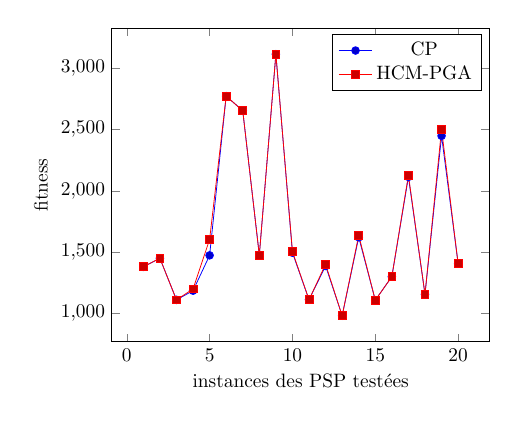
\begin{tikzpicture}[scale=0.7]
       	\begin{axis}[xlabel=instances des PSP testées, ylabel=fitness]
        %\addplot {x^2+2*x-1};
        \addplot coordinates {
        	(1 ,1377)
        	(2 ,1447)
        	(3 ,1107)
        	(4 ,1182)
        	(5 ,1471)
       		(6 ,2774)
       		(7 ,2655)
        	(8 ,1473)
        	(9 ,3117)
        	(10 ,1493)
        	(11 ,1108)
        	(12 ,1384)
        	(13 ,977)
        	(14 ,1619)
        	(15 ,1104)
        	(16 ,1297)
        	(17 ,2113)
        	(18 ,1152)
        	(19 ,2449)
        	(20 ,1403)
        	};
        \addlegendentry{CP}
        \addplot coordinates {
        	(1 ,1378)
        	(2 ,1447)
        	(3 ,1107)
        	(4 ,1196)
        	(5 ,1601)
       		(6 ,2774)
       		(7 ,2655)
        	(8 ,1473)
        	(9 ,3117)
        	(10 ,1502)
        	(11 ,1108)
        	(12 ,1398)
        	(13 ,977)
        	(14 ,1635)
        	(15 ,1104)
        	(16 ,1297)
        	(17 ,2127)
        	(18 ,1152)
        	(19 ,2503)
        	(20 ,1403)
        	};
        \addlegendentry{HCM-PGA}
        \end{axis}
        %\caption{g}
    \end{tikzpicture}
    \end{center}
    \caption{Performances comparées de CP et HCM-PGA en fitness de la meilleure solution trouvée}
    \label{fig:CP_HCM-PGA_best_fitness}
    \end{figure}	
	
	Nous analysons ensuite la performance de HCM-PGA en matière de temps de la meilleure solution trouvée sur nos 10 essais; comme le montre la figure \ref{fig:CP_HCM-PGA_time}, avec pour critère de comparaison le temps de recherche. Nous constatons que le HCM-PGA parcourt bien plus vite l'espace de recherche. Il nous est possible de constater que sur certaines instances le gain de temps est dans le meilleur des cas (instance 10) de 97,21\% . En poursuivant notre analyse, nous pouvons  également faire noter que le temps de recherche est relativement constant. Sur des instances où l'approche CP prend beaucoup plus de temps (instances 6,7,8,9 et 10), notre méthode HCM-PGA conserve un temps de recherche stable. En conséquence, l'usage de notre méthode HCM-PGA s'avère pertinent car elle permet d'avoir sur ces instances, des solutions de bonnes qualités assez rapidement.	
	
	\begin{figure}[!h]
	\begin{center}
	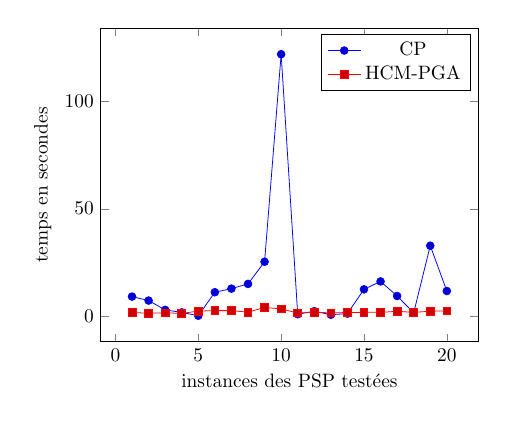
\begin{tikzpicture}[scale=0.7]
       	\begin{axis}[xlabel=instances des PSP testées, ylabel=temps en secondes]
        \addplot coordinates {
        	(1 ,9.14)
        	(2 ,7.29)
        	(3 ,2.94)
        	(4 ,1.78)
        	(5 ,0.23)
       		(6 ,11.17)
       		(7 ,12.84)
        	(8 ,15.03)
        	(9 ,25.35)
        	(10 ,121.90)
        	(11 ,0.935)
        	(12 ,2.347)
        	(13 ,0.711)
        	(14 ,1.223)
        	(15 ,12.508)
        	(16 ,16.187)
        	(17 ,9.404)
        	(18 ,1.589)
        	(19 ,32.811)
        	(20 ,11.726)
        	};
        \addlegendentry{CP}
        \addplot coordinates {
        	(1 ,1.73)
        	(2 ,1.4)
        	(3 ,1.6)
        	(4 ,1.3)
        	(5 ,2.4)
       		(6 ,2.6)
       		(7 ,2.6)
        	(8 ,1.9)
        	(9 ,4.08)
        	(10 ,3.4)
        	(11 ,1.5)
        	(12 ,1.8)
        	(13 ,1.6)
        	(14 ,1.7)
        	(15 ,1.8)
        	(16 ,1.8)
        	(17 ,2.3)
        	(18 ,1.8)
        	(19 ,2.32)
        	(20 ,2.5)
        	};
        \addlegendentry{HCM-PGA}
        \end{axis}
        %\caption{g}
    \end{tikzpicture}
    \caption{Performances comparées de CP et HCM-PGA en temps}
    \label{fig:CP_HCM-PGA_time}
    \end{center}
    \end{figure}
    
    \hspace*{.5cm} En combinant cette analyse ainsi que la précédente, nous pouvons déduire que notre solution HCM-PGA réussit à parcourir l'espace de recherche plus vite que notre approche de référence tout en réussissant sur nos 10 essais tests à trouver une solution optimale ou une solution approchant cette dernière de très près; excepté d'autres instances (instance 5). Nous allons pour la suite, analyser la moyenne des solutions trouvées en matière de performance de fitness.
    
	Trouver une solution proche ou exacte sur un essai est une chose. Arriver à prouver que notre approche trouve des solutions voisines ou proches à la solution exacte sur de nombreux essais est encore une autre chose. La figure \ref{fig:CP_HCM-PGA_moy_fitness} nous permet de dire que notre méthode HCM-PGA peut être efficace dans la résolution des 20 instances présentées et plus largement des instances proposées par Houndji.
    
    \begin{figure}[!h]
    \begin{center}
	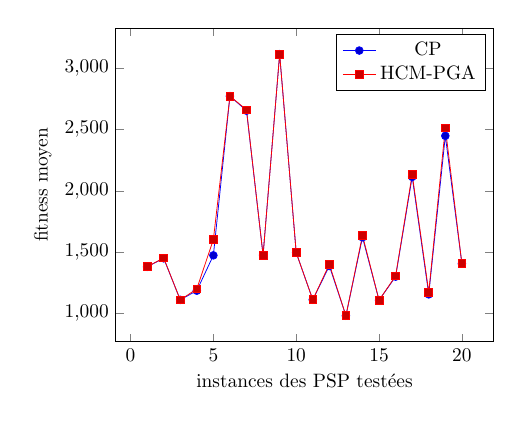
\begin{tikzpicture}[scale=0.7]
       	\begin{axis}[xlabel=instances des PSP testées, ylabel=fitness moyen]
        %\addplot {x^2+2*x-1};
        \addplot coordinates {
        	(1 ,1377)
        	(2 ,1447)
        	(3 ,1107)
        	(4 ,1182)
        	(5 ,1471)
       		(6 ,2774)
       		(7 ,2655)
        	(8 ,1473)
        	(9 ,3117)
        	(10 ,1493)
        	(11 ,1108)
        	(12 ,1384)
        	(13 ,977)
        	(14 ,1619)
        	(15 ,1104)
        	(16 ,1297)
        	(17 ,2113)
        	(18 ,1152)
        	(19 ,2449)
        	(20 ,1403)
        	};
        \addlegendentry{CP}
        \addplot coordinates {
        	(1 ,1378)
        	(2 ,1450)
        	(3 ,1107)
        	(4 ,1196)
        	(5 ,1601)
       		(6 ,2774)
       		(7 ,2662)
        	(8 ,1473)
        	(9 ,3117)
        	(10 ,1493)
        	(11 ,1108)
        	(12 ,1398)
        	(13 ,977)
        	(14 ,1635)
        	(15 ,1104)
        	(16 ,1303)
        	(17 ,2134)
        	(18 ,1171)
        	(19 ,2515)
        	(20 ,1403)
        	};
        \addlegendentry{HCM-PGA}
        \end{axis}
        %\caption{g}
    \end{tikzpicture}
    \end{center}
    \caption{Performances comparées de CP et HCM-PGA en fitness moyen des solutions trouvées}
    \label{fig:CP_HCM-PGA_moy_fitness}
	\end{figure}    
	
    
	\subsection{HFC-PGA et Approche CP}
		Une fois, notre première approche HCM-PGA vérifiée pour les instances proposées par Houndji; nous passons à la seconde méthode de HFC-PGA. La procédure utilisée est similaire à celle utilisée afin de vérifier notre approche HCM-PGA. Nous avons donc analysé les performances en terme de qualité des solutions fournies par notre méthode HFC-PGA. La figure \ref{fig:CP_HFC-PGA_best_fitness} présente les courbes des deux méthodes CP et HFC-PGA. Il en ressort que notre approche HFC-PGA est aussi efficace que l'approche CP. En effet, la déviation maximale sur les 20 instances testées est de  3,2\% (instance 90). Nous estimons cette déviation comme faible. Ainsi, nous pouvons dire que les performances en qualité des meilleures solutions obtenues de l'approche HFC-PGA sont sensiblement égales à celles obtenues de l'approche CP.
    
    \begin{figure}[!h]
    \begin{center}
	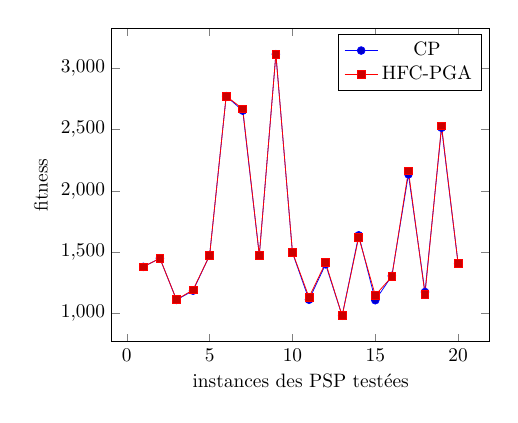
\begin{tikzpicture}[scale=0.7]
       	\begin{axis}[xlabel=instances des PSP testées, ylabel=fitness]
        %\addplot {x^2+2*x-1};
        \addplot coordinates {
        	(1 ,1377)
        	(2 ,1447)
        	(3 ,1107)
        	(4 ,1182)
        	(5 ,1471)
       		(6 ,2774)
       		(7 ,2655)
        	(8 ,1473)
        	(9 ,3117)
        	(10 ,1493)
        	(11 ,1108)
        	(12 ,1398)
        	(13 ,977)
        	(14 ,1635)
        	(15 ,1104)
        	(16 ,1303)
        	(17 ,2134)
        	(18 ,1171)
        	(19 ,2515)
        	(20 ,1403)
        	};
        \addlegendentry{CP}
        \addplot coordinates {
        	(1 ,1377)
        	(2 ,1447)
        	(3 ,1108)
        	(4 ,1189)
        	(5 ,1471)
       		(6 ,2774)
       		(7 ,2670)
        	(8 ,1473)
        	(9 ,3117)
        	(10 ,1497)
        	(11 ,1128)
        	(12 ,1411)
        	(13 ,977)
        	(14 ,1619)
        	(15 ,1145)
        	(16 ,1297)
        	(17 ,2162)
        	(18 ,1152)
        	(19 ,2531)
        	(20 ,1403)
        	};
        \addlegendentry{HFC-PGA}
        \end{axis}
    \end{tikzpicture}
    \end{center}
	\caption{Performances comparées de CP et HFC-PGA en fitness de la meilleure solution trouvée}
	\label{fig:CP_HFC-PGA_best_fitness}
    \end{figure}
    
	La figure \ref{fig:CP_HFC-PGA_time} nous présente les résultats en temps des essais de l'approche HFC-PGA comparés à ceux de l'approche CP. Ainsi, l'approche HFC-PGA parcourt également bien plus vite l'espace de recherche en comparaison à l'approche CP. Un gain de 94,67\% est notamment constaté sur l'instance 10 justifiant la performance en temps de notre solution.    
    
	\begin{figure}[!h]
	
	\begin{center}
	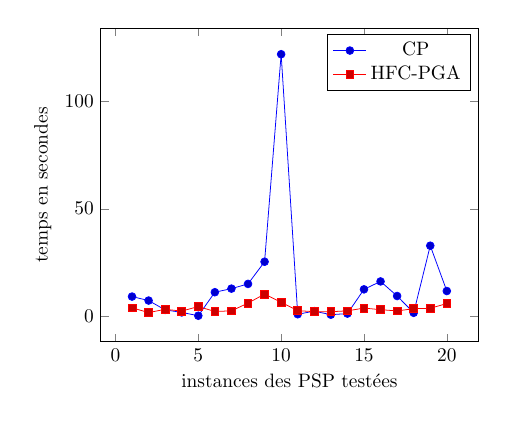
\begin{tikzpicture}[scale=0.7]
       	\begin{axis}[xlabel=instances des PSP testées, ylabel=temps en secondes]
        %\addplot {x^2+2*x-1};
        \addplot coordinates {
        	(1 ,9.14)
        	(2 ,7.29)
        	(3 ,2.94)
        	(4 ,1.78)
        	(5 ,0.23)
       		(6 ,11.17)
       		(7 ,12.84)
        	(8 ,15.03)
        	(9 ,25.35)
        	(10 ,121.90)
        	(11 ,0.935)
        	(12 ,2.347)
        	(13 ,0.711)
        	(14 ,1.223)
        	(15 ,12.508)
        	(16 ,16.187)
        	(17 ,9.404)
        	(18 ,1.589)
        	(19 ,32.811)
        	(20 ,11.726)
        	};
        \addlegendentry{CP}
        \addplot coordinates {
        	(1 ,3.9)
        	(2 ,1.7)
        	(3 ,3.2)
        	(4 ,2.4)
        	(5 ,4.5)
       		(6 ,2.2)
       		(7 ,2.5)
        	(8 ,6.1)
        	(9 ,10.3)
        	(10 ,6.5)
        	(11 ,2.6)
        	(12 ,2.11)
        	(13 ,2.1)
        	(14 ,2.5)
        	(15 ,3.8)
        	(16 ,3.04)
        	(17 ,2.47)
        	(18 ,3.5)
        	(19 ,3.7)
        	(20 ,5.9)
        	};
        \addlegendentry{HFC-PGA}
        \end{axis}
        %\caption{g}
    \end{tikzpicture}
    \end{center}
	\caption{Performances comparées de CP et HFC-PGA en temps}
	\label{fig:CP_HFC-PGA_time}
    \end{figure}
	
	
	Afin de vérifier que notre méthode arrive à trouver en général des solutions proches de la solution optimale, une moyenne de résultats obtenus a été effectuée sur les 10 essais de test. Comme le montre la figure \ref{fig:CP_HFC-PGA_moy_fitness} qui présente les courbes des résultats moyens en terme de qualité du HFC-PGA; nous pouvons remarquer que notre méthode arrive à trouver sur les différents essais effectués des solutions très proches de la solution optimale. En effet, la déviation maximale observée est de 3,3\%. Des observations précédentes et de celle-ci, nous pouvons dire que notre méthode HFC-PGA comme sa seconde HCM-PGA parcourt bien plus vite l'espace de recherche tout en trouvant de solutions optimales sinon très proches de ces dernières.
    \begin{figure}[!h]
    \begin{center}
	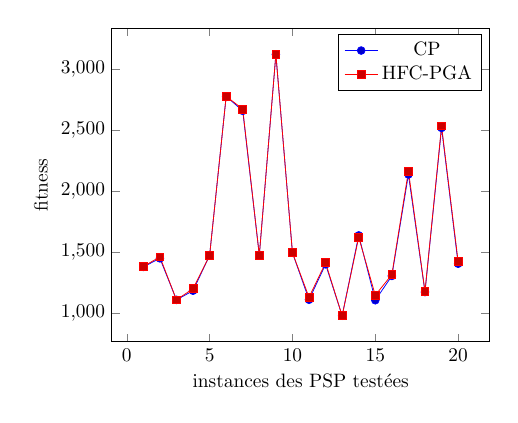
\begin{tikzpicture}[scale=0.7]
       	\begin{axis}[xlabel=instances des PSP testées, ylabel=fitness]
        %\addplot {x^2+2*x-1};
        \addplot coordinates {
        	(1 ,1377)
        	(2 ,1447)
        	(3 ,1107)
        	(4 ,1182)
        	(5 ,1471)
       		(6 ,2774)
       		(7 ,2655)
        	(8 ,1473)
        	(9 ,3117)
        	(10 ,1493)
        	(11 ,1108)
        	(12 ,1398)
        	(13 ,977)
        	(14 ,1635)
        	(15 ,1104)
        	(16 ,1303)
        	(17 ,2134)
        	(18 ,1171)
        	(19 ,2515)
        	(20 ,1403)
        	};
        \addlegendentry{CP}
        \addplot coordinates {
        	(1 ,1380)
        	(2 ,1459)
        	(3 ,1107)
        	(4 ,1199)
        	(5 ,1471)
       		(6 ,2774)
       		(7 ,2670)
        	(8 ,1473)
        	(9 ,3119)
        	(10 ,1493)
        	(11 ,1128)
        	(12 ,1411)
        	(13 ,977)
        	(14 ,1619)
        	(15 ,1145)
        	(16 ,1314)
        	(17 ,2162)
        	(18 ,1177)
        	(19 ,2531)
        	(20 ,1422)
        	};
        \addlegendentry{HFC-PGA}
        \end{axis}
        %\caption{g}
    \end{tikzpicture}
    \end{center}
    \caption{Performances comparées de CP et HFC-PGA en fitness moyen des solutions trouvées}
    \label{fig:CP_HFC-PGA_moy_fitness}
    \end{figure}
    

		\subsection{HCM-PGA et Approche SA}
		
		Les analyses précédentes nous ont permis de dire que nos deux approches basées sur les algorithmes génétiques performent aussi bien en qualité que l'approche CP, tout en parcourant bien plus vite l'espace de recherche. Nous allons dans la suite tenter d'analyser les résultats issus des tests effectués sur des instances bien plus grandes de la bibliothèque Opthub. Ces instances sont en effet plus grandes avec leur horizon de planification supérieur à 200 périodes. La figure \ref{fig:SA_HCM-PGA_time} montre les courbes décrivant l'allure des résultats en temps des deux approches HCM-PGA et SA; et nous permet ainsi de comparer les résultats obtenus. \\
		\hspace*{.5cm} Sur les figures en rapport à l'approche SA, les numéros 1,2,3,4,5 et 6 correspondent respectivement aux instances ps-200-10-80, ps-200-20-80, ps-300-10-80, ps-300-20-80, ps-400-10-80 et ps-400-20-80.
		
		
	\begin{figure}[!h]
    \begin{center}
	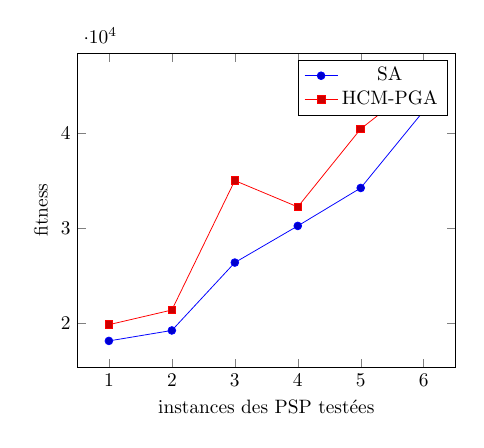
\begin{tikzpicture}[scale=0.7]
       	\begin{axis}[xlabel=instances des PSP testées, ylabel=fitness]
        %\addplot {x^2+2*x-1};
        \addplot coordinates {
        	(1 ,18089)
        	(2 ,19190)
        	(3 ,26343)
        	(4 ,30206)
        	(5 ,34206)
       		(6 ,42329)
        	};
        \addlegendentry{SA}
        \addplot coordinates {
        	(1 ,19799)
        	(2 ,21345)
        	(3 ,34985)
        	(4 ,32207)
        	(5 ,40433)
       		(6 ,45647)
        	};
        \addlegendentry{HCM-PGA}
        \end{axis}
    \end{tikzpicture}
    \end{center}
	\caption{Performances comparées de SA et HCM-PGA en fitness de la meilleure solution trouvée}
	\label{fig:SA_HCM-PGA_best_fitness}
    \end{figure}	
    
	En observant la figure \ref{fig:SA_HCM-PGA_best_fitness}, on constate que les résultats de notre méthode HCM-PGA diffèrent nettement de celles optimales de la méthode SA. On remarque en effet, que la méthode de résolution HCM-PGA trouve des solutions dont le coût est différent de 32\% dans le pire des cas (instance ps-300-10-80). Nous pouvons cependant retenir comme point positif que notre méthode HCM-PGA réussit à approcher de 6.6\% dans le meilleur des cas (instance ps-300-20-80) la solution optimale.
	
	\begin{figure}[!h]
	\begin{center}
	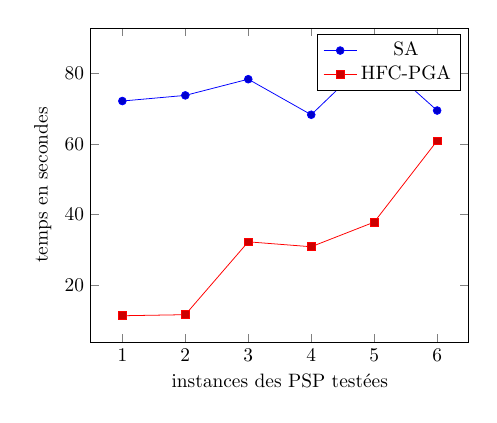
\begin{tikzpicture}[scale=0.7]
       	\begin{axis}[xlabel=instances des PSP testées, ylabel=temps en secondes]
        %\addplot {x^2+2*x-1};
        \addplot coordinates {
        	(1 ,72.2)
        	(2 ,73.8)
        	(3 ,78.4)
        	(4 ,68.3)
        	(5 ,85.5)
       		(6 ,69.5)
        	};
        \addlegendentry{SA}
        \addplot coordinates {
        	(1 ,11.2)
        	(2 ,11.5)
        	(3 ,32.2)
        	(4 ,30.8)
        	(5 ,37.8)
       		(6 ,60.9)
        	};
        \addlegendentry{HFC-PGA}
        \end{axis}
        %\caption{g}
    \end{tikzpicture}
    \end{center}
	\caption{Performances comparées de SA et HCM-PGA en temps}
	\label{fig:SA_HCM-PGA_time}
    \end{figure} 
    
	Notons que notre méthode HCM-PGA ne performe pas aussi bien qu'attendu sur les instances plus grandes lorsqu'on parle de qualité de la meilleure solution trouvée. Nous analysons à présent ses performances en temps. La figure \ref{fig:SA_HCM-PGA_time} nous indique que notre méthode HCM-PGA parcourt toujours aussi vite l'espace de recherche (jusqu'à 84\% de gain en temps dans le meilleur des cas). Nous résumons donc de nos deux analyses en terme de temps et de qualité, que notre méthode HCM-PGA explore toujours aussi vite l'espace de recherche mais ne réussit pas à mieux approcher la solution au delà de 6.6\%.    
    
 
    \subsection{HFC-PGA et Approche SA}	

	La figure \ref{fig:SA_HFC-PGA_best_fitness} présente les résultats des tests effectués en terme de qualité de la solution trouvée. Une analyse similaire à celle menée entre SA et HCM-PGA peut être menée dans le sens où les performances en terme de qualité des solutions obtenues des essais de la méthode HFC-PGA sur les 6 instances plus grandes, ne sont pas aussi intéressantes qu’espérées. En effet, notre méthode de HFC-PGA ne fait pas mieux que 6.4\% dans le meilleur des cas (instance ps-300-20-80). Il est à noter cependant comme point positif que notre méthode HFC-PGA ne fait pas moins bien que 19.2\% de déviation maximale. 
	
	\begin{figure}[!h]
    \begin{center}
	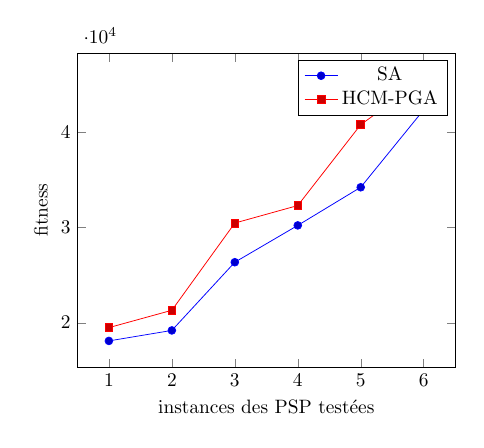
\begin{tikzpicture}[scale=0.7]
       	\begin{axis}[xlabel=instances des PSP testées, ylabel=fitness]
        %\addplot {x^2+2*x-1};
        \addplot coordinates {
        	(1 ,18089)
        	(2 ,19190)
        	(3 ,26343)
        	(4 ,30206)
        	(5 ,34206)
       		(6 ,42329)
        	};
        \addlegendentry{SA}
        \addplot coordinates {
        	(1 ,19484)
        	(2 ,21302)
        	(3 ,30452)
        	(4 ,32289)
        	(5 ,40775)
       		(6 ,45521)
        	};
        \addlegendentry{HCM-PGA}
        \end{axis}
    \end{tikzpicture}
    \end{center}
	\caption{Performances comparées de SA et HFC-PGA en fitness de la meilleure solution trouvée}
	\label{fig:SA_HFC-PGA_best_fitness}
    \end{figure} 	
	
	Du point de vue de la performance en temps de notre méthode comparée à la méthode SA, plus l'horizon de planification s'étend plus, l'efficacité en temps se dégrade. En effet, elle est de 9.9 secondes sur un horizon de 200 périodes et de 120 secondes sur un horizon de 400 périodes; environ deux fois plus que le temps pris par la méthode SA pour cette dernière instance comme le montre la figure \ref{fig:SA_HFC-PGA_time}.
	\begin{figure}[!h]
	\begin{center}
	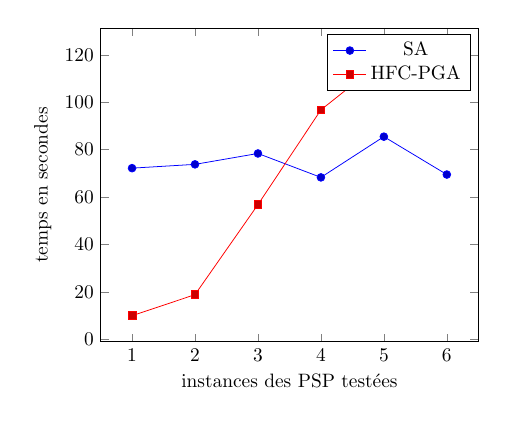
\begin{tikzpicture}[scale=0.7]
       	\begin{axis}[xlabel=instances des PSP testées, ylabel=temps en secondes]
        %\addplot {x^2+2*x-1};
        \addplot coordinates {
        	(1 ,72.2)
        	(2 ,73.8)
        	(3 ,78.4)
        	(4 ,68.3)
        	(5 ,85.5)
       		(6 ,69.5)
        	};
        \addlegendentry{SA}
        \addplot coordinates {
        	(1 ,9.9)
        	(2 ,18.8)
        	(3 ,56.8)
        	(4 ,96.8)
        	(5 ,117.9)
       		(6 ,120.3)
        	};
        \addlegendentry{HFC-PGA}
        \end{axis}
        %\caption{g}
    \end{tikzpicture}
    \end{center}
	\caption{Performances comparées de SA et HFC-PGA en temps}
	\label{fig:SA_HFC-PGA_time}
    \end{figure}
        	
    
		\subsection{HCM-PGA et HFC-PGA}

	Dans cette section, nous tentons de répondre à la question de savoir laquelle des méthodes HCM-PGA et HFC-PGA est la plus pertinente dans la résolution des problèmes du PSP en nous basant sur les résultats des tests effectués sur les instances proposées par Houndji. Les figures \ref{fig:HCM-PGA_HFC-PGA_time} et \ref{fig:HCM-PGA_HFC-PGA_moy_fitness} présentent respectivement les résultats en terme de temps et de qualité. On note ainsi globalement que la méthode de HCM-PGA est plus rapide que celle du HFC-PGA et également plus précise que cette dernière lorsqu’on parle de qualité des solutions trouvées. Nous nous expliquons cela sans doute par le fait que les algorithmes génétiques parallèles et hiérarchiques HFC-PGA doivent faire démarrer un grand nombre de nœuds (ou threads) correspondants chacune à un chromosome afin de pouvoir explorer l'espace de recherche ainsi qu'à la topologie utilisée dans le HFC-PGA.
		
		
	\begin{figure}[!h]
	\begin{center}
	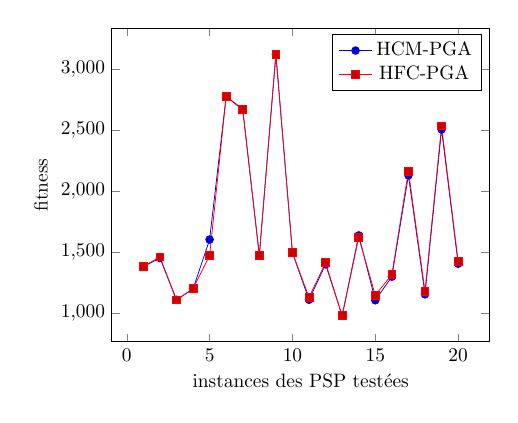
\begin{tikzpicture}[scale=0.7]
       	\begin{axis}[xlabel=instances des PSP testées, ylabel=fitness]
        %\addplot {x^2+2*x-1};
        \addplot coordinates {
        	(1 ,1378)
        	(2 ,1450)
        	(3 ,1107)
        	(4 ,1196)
        	(5 ,1601)
       		(6 ,2774)
       		(7 ,2662)
        	(8 ,1473)
        	(9 ,3117)
        	(10 ,1493)
        	(11 ,1108)
        	(12 ,1398)
        	(13 ,977)
        	(14 ,1635)
        	(15 ,1104)
        	(16 ,1297)
        	(17 ,2127)
        	(18 ,1152)
        	(19 ,2503)
        	(20 ,1403)
        	};
        \addlegendentry{HCM-PGA}
        \addplot coordinates {
        	(1 ,1380)
        	(2 ,1459)
        	(3 ,1107)
        	(4 ,1199)
        	(5 ,1471)
       		(6 ,2774)
       		(7 ,2670)
        	(8 ,1473)
        	(9 ,3119)
        	(10 ,1493)
        	(11 ,1128)
        	(12 ,1411)
        	(13 ,977)
        	(14 ,1619)
        	(15 ,1145)
        	(16 ,1314)
        	(17 ,2162)
        	(18 ,1177)
        	(19 ,2531)
        	(20 ,1422)
        	};
        \addlegendentry{HFC-PGA}
        \end{axis}
        %\caption{g}
    \end{tikzpicture}
    \end{center}
    \caption{Performances comparées de HCM-PGA et HFC-PGA en fitness moyen des solutions trouvées}
    \label{fig:HCM-PGA_HFC-PGA_moy_fitness}
    \end{figure}
    
    \begin{figure}[!h]
	
	\begin{center}
	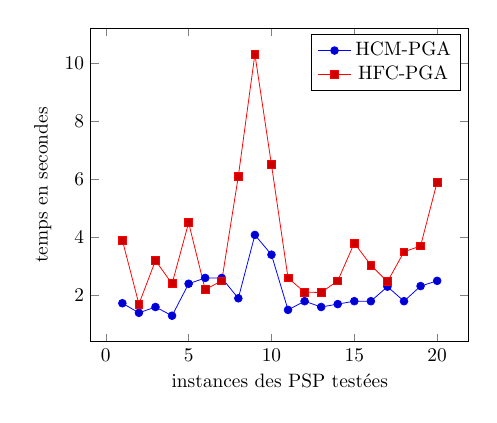
\begin{tikzpicture}[scale=0.7]
       	\begin{axis}[xlabel=instances des PSP testées, ylabel=temps en secondes]
        %\addplot {x^2+2*x-1};
        \addplot coordinates {
        	(1 ,1.73)
        	(2 ,1.4)
        	(3 ,1.6)
        	(4 ,1.3)
        	(5 ,2.4)
       		(6 ,2.6)
       		(7 ,2.6)
        	(8 ,1.9)
        	(9 ,4.08)
        	(10 ,3.4)
        	(11 ,1.5)
        	(12 ,1.8)
        	(13 ,1.6)
        	(14 ,1.7)
        	(15 ,1.8)
        	(16 ,1.8)
        	(17 ,2.3)
        	(18 ,1.8)
        	(19 ,2.32)
        	(20 ,2.5)
        	};
        \addlegendentry{HCM-PGA}
        \addplot coordinates {
        	(1 ,3.9)
        	(2 ,1.7)
        	(3 ,3.2)
        	(4 ,2.4)
        	(5 ,4.5)
       		(6 ,2.2)
       		(7 ,2.5)
        	(8 ,6.1)
        	(9 ,10.3)
        	(10 ,6.5)
        	(11 ,2.6)
        	(12 ,2.11)
        	(13 ,2.1)
        	(14 ,2.5)
        	(15 ,3.8)
        	(16 ,3.04)
        	(17 ,2.47)
        	(18 ,3.5)
        	(19 ,3.7)
        	(20 ,5.9)
        	};
        \addlegendentry{HFC-PGA}
        \end{axis}
    \end{tikzpicture}
    \end{center}
    
	\caption{Performances comparées de HCM-PGA et HFC-PGA en temps}
	\label{fig:HCM-PGA_HFC-PGA_time}
    \end{figure} 
    
		\section*{Conclusion}
		\addcontentsline{toc}{section}{Conclusion}
		Les tests effectués dans cette partie ont été l'occasion de vérifier nos deux méthodes de résolution proposées basées sur les algorithmes génétiques. Nous avons ainsi pu comparer chacune d'elles aux approches CP et SA et avons pu tirer des conclusions. Il ne nous reste plus qu'à conclure notre étude et à présenter les perspectives envisagées.

%%conclusion
\lhead[]{} \rhead[]{} \chead[]{}
\conclusion
	
Nous avons présenté	les problèmes de dimensionnement de lots. Nous avons montré que la résolution de ces types de problèmes soulève certains défis intéressants. Nous nous sommes en particulier intéressés au \emph{Pigment Sequencing Problem} (PSP). Plusieurs méthodes de résolution du PSP ont été testées au cours de récentes recherches. Il s'agit des approches MIP, CP et SA. Cependant, aucune approche basée sur les algorithmes génétiques n'avait été proposée alors que ces derniers ont montré leur efficacité sur d'autres problèmes d'optimisation.\\
	\hspace*{.5cm} Nous avons proposé deux méthodes de résolution du PSP en utilisant les algorithmes génétiques parallèles hiérarchiques : \emph{Hierarchical Coarse-grained and Master-slave Parallel Genetic Algorithm} (HCM-PGA) et \emph{Hierarchical Fine-grained and Coarse-grained Parallel Genetic Algorithm}(HFC-PGA). L'approche HCM-PGA divise la population globale en sous-populations ou îlots auxquels sont appliquées les opérations génétiques telles le croisement, la mutation ainsi que la sélection. Également, l'approche HCM-PGA confie à différents nœuds ou threads la tâche d'appliquer les opérations génétiques les plus gourmandes en ressource afin d'accélérer la recherche. Quant à l'approche HFC-PGA, elle divise dans la même logique la population globale en sous-populations; ces dernières étant disposées suivant une topologie de connexion particulière favorisant le chevauchement des bons chromosomes et la dissémination du matériel génétique. Nous avons vérifié nos deux propositions de méthodes de résolution à travers des tests que nous avons effectués sur deux groupes d'instances. Le premier est proposé dans la bibliothèque CSPlib et le second dans la bibliothèque Opthub. Ces tests ont permis d'analyser le comportement de nos deux propositions et de dire qu'elles parviennent en un temps raisonnable à trouver de solutions approchant la solution optimale en particulier sur les instances dont l'horizon de planification est inférieur ou égal à 20 périodes.\\
	\hspace*{.5cm}Le travail présenté dans ce document est un bon point de départ pour de futurs développements et extensions utilisant les algorithmes génétiques. Il serait par exemple intéressant de penser à des algorithmes de recherche locale qui améliorent significativement la qualité d'un chromosome tout en étant rapides sur les chromosomes des grandes instances testées dans notre étude. D'un autre côté, le croisement est un aspect très important dans la résolution des problèmes. Une perspective intéressante est de penser à des moyens de croisement plus intelligents qui améliorent la population. Enfin, l'application des algorithmes génétiques parallèles et hiérarchiques à des problèmes encore plus complexes à plusieurs machines ou à plusieurs niveaux est un sujet intéressant pour de futurs travaux. 

%%biblio
\bibliographystyle{plain} 
\bibliography{main}
%

\appendix
\chapter{Annexe 1}

\section{Classes et implémentation}
	
	Nous présentons ici la structure et quelques classes du programme (HFC-PGA) et nous détaillons les codes de quelques fonctions utilisées.
	
	\subsection{Classes}
	
	\begin{lstlisting}[language=python]
	#Classe représentant un chromosome	
	
class Chromosome(object):

	mutationRate = 0
	problem = 0
	hashTable = {}

	# Builder 
	def __init__(self):
		# Fonction d'initialisation de chromosome
	
	def init2(self, solution, itemsRank):
		# Autre fonction d'initialisation de chromosome
	
	def __lt__(self, chromosome):
		# Fonction utilisée dans le comparaison entre deux chromosomes
	
	def _get_fitnessValue(self):
		# Fonction de calcul du fitness d'un chromosome
	
	def _get_solution(self):
		# Fonction de récupération du genotype d'un chromosome
	
	def _get_itemsRanks(self):
		# Fonction de récupération de la période de satisfaction d'une production
	
	def _get_hashSolution(self):
		# Fonction de récupération du hash du génotype
	
	def _set_hashSolution(self, new_value):
		# Fonction d'attribution du hash d'un genotype
	
	def _set_itemsRanks(self, new_value):
		# Fonction d'attribution de la liste des rangs des productions
	
	def _set_solution(self, new_solution):
		# Fonction d'attribution du genotype d'un chromosome
	
	def _set_fitnessValue(self, new_value):
		# Fonction d'attribution de la valeur de fitness a un chromosome
	
	def __repr__(self):
		# Fonction d'affichage d'un chromosome
	
	def __eq__(self, chromosome):
		# Fonction utilisée dans le comparaison entre deux chromosomes
	
	def __ne__(self, chromosome):
		# Fonction utilisée dans le comparaison entre deux chromosomes
	
	def isFeasible(self):
		# Fonction de vérification de la faisabilité d'un chromosome
	
	def mutate(self):
		# Fonction utilisée afin de faire muter un chromosome
	
	def advmutate(self):
		# Fonction utilisée comme fonction de recherche locale
	
	def getFeasible(self):
		# Fonction utilisée afin de rendre faisable un chromosome
	
	def getCostof(cls, indice, item, rank,solution, secondIndice = -1):
		# Fonction de détermination du cout d'un gene dans le génotype d'un chromosome
	
	# Class' methods
	getCostof = classmethod(getCostof)

	# Properties
	solution = property(_get_solution,_set_solution)
	fitnessValue = property(_get_fitnessValue,_set_fitnessValue)
	itemsRank = property(_get_itemsRanks, _set_itemsRanks)
	hashSolution = property(_get_hashSolution, _set_hashSolution) 

    \end{lstlisting}
    
    \begin{lstlisting}[language=python]
    // Classe représentant un thread principal en HFC-PGA
    
class ClspThread(Thread):

	listMainThreads = 0
	NumberOfMigrants = 0
	NbGenToStop = 0
	crossOverRate = 0
	MigrationRate = 0
	NbMaxPopulation = 0
	FITNESS_PADDING = 0

	def __init__(self, threadId):
		# Constructeur de la classe	
	
	def run(self):
		# Fonction d'exécution du thread	
	
	def getPopImproved(self):
		# Fonction utilisée dans l'amélioration de la qualité de la population initiale	
	
	def exploit(self, chromosome):
		# Fonction utilisée afin d'exploiter un chromosome apres exploration 
		
	def initSearch(self, queue, parameter = "main"):
		# Fonction d'execution de la formation de la population initiale	
	
	def sendMigrants(self):
		# Fonction utilisee afin d'envoyer des chromosomes aux threads voisins	
	
	def receiveMigrants(self, chromosomes):
		# Fonction utilisee dans la reception des chromosomes de threads voisins	
	
	def replace(self, chromosome):
		#Code de la fonction ici	
	
	def getFitnessData(self):
		# Fonction utilisee dans la procedure de Roulette Wheel	
	
	def mate(self, chromosome1, chromosome2):
		# Fonction utilisee afin de reproduire deux chromosomes	
	
	def crossover(self, randValue1, randValue2):
		# Fonction utilisee dans le croisement de deux chromosomes
	
	def crossPopulation(self):
		# Fonction utilisee afin de lancer le croisement a travers toute la population	

	def insert(self, chromosome):
		# Fonction utilisee afin d'inserer un chromosome dans la population initiale	
		
		
    \end{lstlisting}
    
    \begin{lstlisting}[language=python]
class GeneticAlgorithm:

	#	Class' variables
	NbMaxPopulation = 25
	mutationRate = 0.05
	crossOverRate = 0.80
	FITNESS_PADDING = 1
	NumberOfMigrants = 1
	MigrationRate = 0 
	nbMainThreads = 3
	nbSlavesThread = 3
	NbGenToStop = 7

	# Builder
	def __init__(self, inst):
		# Constructeur de la classe
	
	def start(self):
		# Fonction utilisée afin de lancer l'exécution de l'algorithme génétique
	
	def printResults(self):
		# Fonction utilisée afin d'afficher les résultats
		
    \end{lstlisting}
	
	\subsection{Fonctions}	
	
	\begin{lstlisting}[language=python]
	# Fonction d'évaluation d'un chromosome
	
def evaluate(cls, sol):
			
		solution = list(sol)

		fitnessValue = 0
		# Calculation of all the change-over costs
		itemsRank = [1] * Chromosome.problem.nbItems
		i = 0
		for gene in solution:
			#print("gene : ", gene, " cost : ", Chromosome.getCostof(i, gene, itemsRank[gene-1], solution))
			fitnessValue += Chromosome.getCostof(i, gene, itemsRank[gene-1], solution)
			if gene != 0:
				itemsRank[gene-1] += 1
			i += 1

return fitnessValue		
    \end{lstlisting}	
	
		\begin{lstlisting}[language=python]
		# Fonction de faisabilité d'un chromosome
		
def getFeasible(self):

		#print(" In Chromosome 1 : ", self._solution)
		#print(self._solution)

		#if self.isFeasible() is False:

		#print(" grid : ", grid)
		copy_solution = list(self._solution)

		# i make sure that the number of goods producted isn't superior to the number expected
		i = 0
		while i < Chromosome.problem.nbTimes:

			if self._solution[i] != 0:

				item = self._solution[i]
				#print(" ok : ", self._solution, self._itemsRank)
				#print(" item picked : ", item)
				rank = self._itemsRank[i]
				#print(i, item-1, rank-1, self.manufactItemsPeriods)
				value = self.manufactItemsPeriods[item-1][rank-1]

				if value == -1:
					itemDemandPeriods = self.manufactItemsPeriods[item-1]
					itemDemandPeriods[rank-1] = i
					#print(" It isn't yet in the tab")
					#print(" == -1 ", item, i, rank)

				else:

					#print(" != -1 ", item, i, rank)
					#print(" It is already in the tab")
					cost1 = Chromosome.getCostof(value, item, rank, copy_solution, i)
					cost2 = Chromosome.getCostof(i, item, rank, copy_solution, value)

					#print(" cost 1 : ", cost1, " cost2 : ", cost2)
					if cost2 < cost1 :
						itemDemandPeriods = self.manufactItemsPeriods[item-1]
						itemDemandPeriods[rank-1] = i

						#print(" cost2 < cost1 : ", value, item)
						self._solution[value] = 0

					else:
						self._solution[i] = 0
			i+=1

		#print(" in middle getFeasible : ", self._solution, ", ", self._itemsRank)
		#print()
		# i make sure that the number of items producted isn't inferior to the number expected
		i = 0
		while i < Chromosome.problem.nbItems:

			j = 0
			nbmanufactItemsPeriods = len(self.manufactItemsPeriods[i])
			while j < nbmanufactItemsPeriods:

				if self.manufactItemsPeriods[i][j] == -1:
					if j == 0:
						lbound = 0
					else:
						lbound = self.manufactItemsPeriods[i][j-1]
					
					zeroperiods = []
					k = lbound+1
					while k <= Chromosome.problem.deadlineDemandPeriods[i][j]:
						if self._solution[k] == 0:
							zeroperiods.append(k)
						k+=1

					#print("zeroperiods : ", zeroperiods)
					nbZeroPeriods = len(zeroperiods)

					if nbZeroPeriods > 0:

						cost1 = Chromosome.getCostof(zeroperiods[0], i+1, j+1, copy_solution)
						#print(" cost1 : ", cost1 )

						k = 1 
						indice = zeroperiods[0]
						while k < nbZeroPeriods:
							cost2 = Chromosome.getCostof(zeroperiods[k], i+1, j+1, copy_solution)
							#print(" cost2 : ", cost2 , zeroperiods[k])
							if cost2 < cost1:
								#print(" cost2 < cost1 : ", cost1 , cost2 )
								indice = zeroperiods[k]
							k+=1

						self._solution[indice] = i+1

						itemDemandPeriods = self.manufactItemsPeriods[i]
						itemDemandPeriods[j] = indice

					else:
						
						# experimental code 

						# if there's no place to put this item, then i check all the other times in order to put this item there
						
						lbound = 0
						p = 1
						for deadline in Chromosome.problem.deadlineDemandPeriods[i]:

							zeroperiods = []
							k = lbound
							while k <= deadline:
								if self._solution[k] == 0:
									zeroperiods.append(k)
								k += 1
							lbound = deadline + 1

							nbZeroPeriods = len(zeroperiods)
							if nbZeroPeriods > 0:

								cost1 = Chromosome.getCostof(zeroperiods[0], i+1, p, copy_solution)
								#print(" cost1 : ", cost1 )

								k = 1 
								indice = zeroperiods[0]
								while k < nbZeroPeriods:
									cost2 = Chromosome.getCostof(zeroperiods[k], i+1, p, copy_solution)
									#print(" cost2 : ", cost2 , zeroperiods[k])
									if cost2 < cost1:
										#print(" cost2 < cost1 : ", cost1 , cost2 )
										indice = zeroperiods[k]
									k+=1

								self._solution[indice] = i+1

								itemDemandPeriods = self.manufactItemsPeriods[i]
								itemDemandPeriods[j] = indice

bre
ak
							p += 1


				j+=1
			i+=1

    \end{lstlisting}


\clearpage
\pagenumbering{gobble}
\setcounter{tocdepth}{1}
\tableofcontents
\addcontentsline{toc}{chapter}{Table des matières}

% i add a last page to put on it a qr code that redirect to the github repository of the projet showed above
\vspace*{1cm}	
	\begin{center}
		\begin{figure}[!h]
			
\includegraphics[scale=.2]{images/thesis_project_qrcode.png}
		\end{figure}
	\end{center}


\end{onehalfspace}
\end{document}

